\section{Penjelasan Implementasi dan Coding}
\subsection{Implementasi}
Arti implementasi menurut KBBI (Kamus Besar Bahasa Indonesia) yaitu pelaksanaan / penerapan. Sedangkan pengertian umum adalah suatu tindakan atau pelaksana rencana yang telah disusun secara cermat dan rinci (matang).Kata implementasi sendiri berasal dari bahasa Inggris \textit{“to implement”}  artinya mengimplementasikan. Tak hanya sekedar aktivitas, implementasi merupakan suatu kegiatan yang direncanakan serta dilaksanakan dengan serius juga mengacu pada norma-norma tertentu guna mencapai tujuan kegiatan.
\par Pendapat lain mengatakan bahwa pengertian implementasi adalah suatu tindakan atau bentuk aksi nyata dalam melaksanakan rencana yang telah dirancang dengan matang. Dengan kata lain, implementasi hanya dapat dilakukan jika sudah ada perencanaan dan bukan hanya sekedar tindakan semata.
\par Dari penjelasan tersebut kita dapat melihat bahwa implementasi bermuara pada mekanisme suatu sistem. Penerapan implementasi harus sesuai dengan perencanaan yang telah dibuat agar hasil yang dicapai sesuai dengan yang diharapkan.
\par Seperti yang disebutkan sebelumnya, implementasi merupakan aktivitas yang dilakukan secara sistematis dan terikat oleh mekanisme untuk mencapai tujuan tertentu. Mengacu pada pengertian implementasi tersebut, adapun beberapa tujuan implementasi adalah sebagai berikut:
\begin{enumerate}
    \item Tujuan utama implementasi adalah untuk melaksanakan rencana yang telah disusun dengan cermat, baik oleh individu maupun kelompok.
    \item Untuk menguji serta mendokumentasikan suatu prosedur dalam penerapan rencana atau kebijakan.
    \item Untuk mewujudkan tujuan-tujuan yang hendak dicapai di dalam perencanaan atau kebijakan yang telah dirancang.
    \item Untuk mengetahui kemampuan masyarakat dalam menerapkan suatu kebijakan atau rencana sesuai dengan yang diharapkan.
    \item Untuk mengetahui tingkat keberhasilan suatu kebijakan atau rencana yang telah dirancang demi perbaikan atau peningkatan mutu.

\end{enumerate}
\subsection{\textit{Coding}}
\par  \textit{Coding} yaitu menulis sekumpulan code sesuai syntax (aturan penulisan) tergantung bahasa pemrograman yang dipakai (python, php, ruby, java, atau yang lainya) dengan bantuan text editor seperti sublime text, atom, notepad, dll. Dengan coding, kita memberikan daftar instruksi kepada komputer sesuai tujuan kita mebuat. Contoh coding yaitu kita melakukan penulisan code untuk membuat website, aplikasi android, dan lain sebagainya.\\

\par Tujuan dari Pengkodean (coding) adalah menjadikan setiap karakter data dalam sebuah informasi digital ke dalam bentuk biner agar dapat ditransmisikan dan bisa melakukan komunikasi data.
Kode-kode yang digunakan dalam komunikasi data pada system computer memiliki perbedaan dari generasi ke generasinya, karena semakin besar dan kompleksnya data yang akan dikirim atau digunakan digunakan.

\section{Implementasi Coding Prototipe}
\par Dalam mengimplementasikan codingan untuk membuat prototipe prediksi ketinggian air (PKA) untuk mendeteksi banjir peringatan banjir ini menggunakan bahasa pemograman C. Dimana bahasa pemograman C ini telah di jelaskan pada bab sebelumnya.\\

\par Untuk lebih mempermudah pemahaman mengenai pemograman bahasa C menggunakan \textit{software} Arduino IDE. Maka terlebih dahulu akan memberikan contoh tentang pemograman bahasa C dasar serta cara install dan penggunaan \textit{software} Arduino IDE.

\subsection{Cara \textit{Install} Arduino IDE dan Penggunaanya}
Hal pertama kali yang harus kita butuhkan adalah board development Arduino, yang berfungsi untuk dapat menginstall Arduino IDE. Dalam tutorial ini menggunakan Arduino IDE untuk sistem operasi Windows 10-64 byte yang berformat \textbf{.exe} . Perhatikan langkah-langkah berikut ini:
\begin{enumerate}
    \item Setalah diunduh, klik dua kali file tersebut sehingga muncul jendela instalasi sebagai berikut :
\begin{figure}[H]
\centering
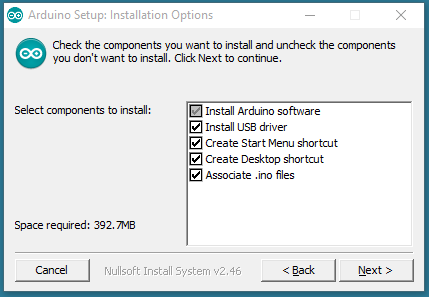
\includegraphics[width=1\textwidth]{figures/ide1.png}
\caption{Tampilan Jendela Instalasi}
\label{print}
\end{figure}
\par Pilih komponen yang sudah diinstal. Sesuaikan dengan kebutuhan anda, pastikan pilihan install USB driver telah tercentang karena ini terkait nanti dengan driver usb Arduino. Setelah beres klik Next.

\item Pada jendela berikutnya akan ditampilkan pada jendela dialog tujuan instalasi dari arduino IDE. Pilih default saja dan langsung klik Install.
\begin{figure}[H]
\centering
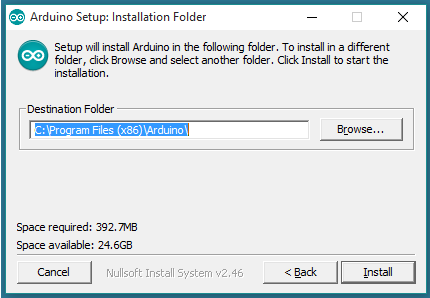
\includegraphics[width=1\textwidth]{figures/ide2.png}
\caption{Jendela Dialog Tujuan Instalasi Dari Arduino IDE }
\label{print}
\end{figure}

\begin{figure}[H]
\centering
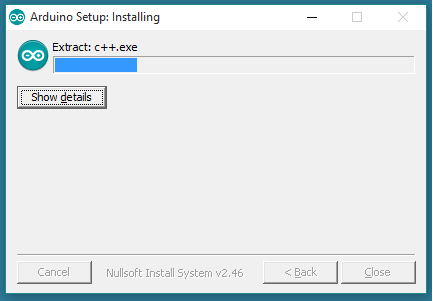
\includegraphics[width=1\textwidth]{figures/ide3.png}
\caption{Jendela Instalasi Arduino IDE }
\label{print}
\end{figure}
\end{enumerate}
\par Tunggu hingga proses instalasi selesei. Setelah Arduino IDE selesei terinstall, kini sambungkan kabel USB Arduino  pada port USB komputer/laptop. Jika anda menggunakan file installer yang sama di tunjukan pada pembahasan sebelumnya, maka arduino akan otomatis terbaca di COMX (X adalah nomer port serial, misalkan COM1 atau COM2 dan seterusnya).

\par Setelah Arduino IDE terinstall maka kita harus \textit{install} juga terlebih dahulu yang diperlukan untuk \textit{development board} NodeMCU. Driver yang dibutuhkan yaitu driver CH34x dan CP210x. Cara mendwonload dan \textit{install} sebagai berikut :
\begin{figure}[H]
\centering
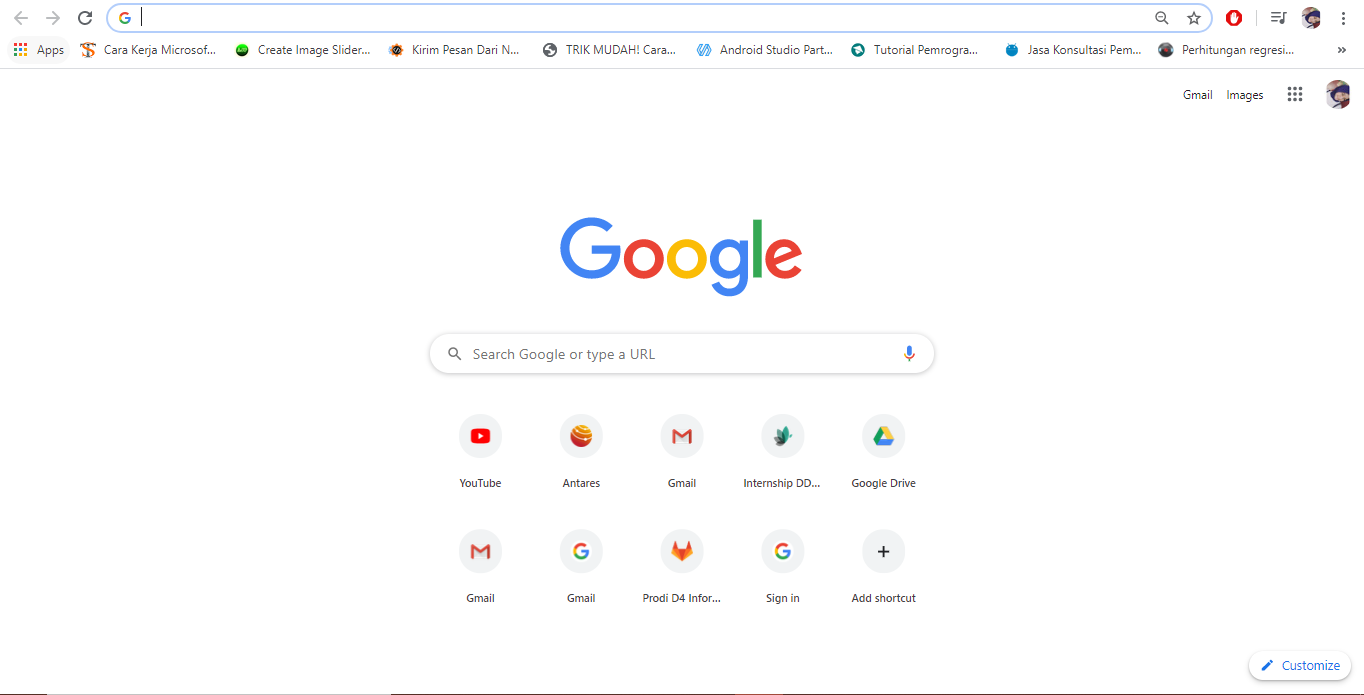
\includegraphics[width=1\textwidth]{figures/google.png}
\caption{Tampilan Google }
\label{print}
\end{figure}

\par Buka browser yang dimiliki, disini menggunakan google. Ketika google di klik maka tampilannya seperti gambar di atas. Setelah itu ketikan Cp210 driver.
\begin{figure}[H]
\centering
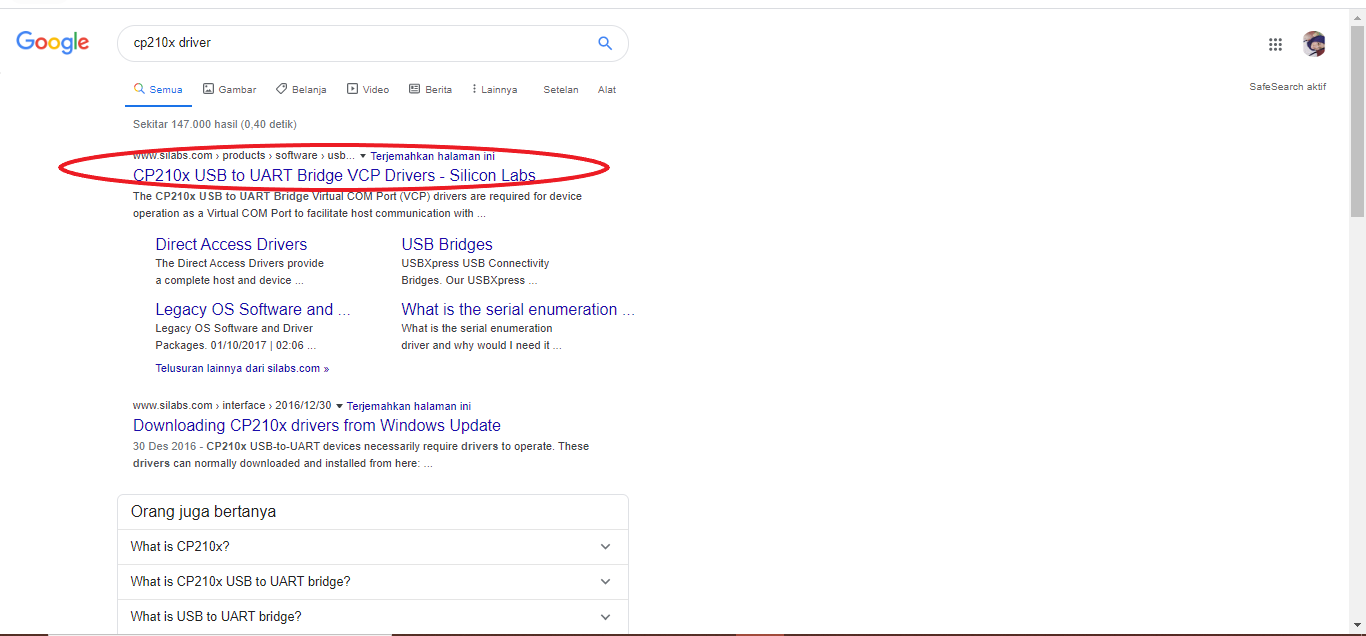
\includegraphics[width=1\textwidth]{figures/google2.png}
\caption{Tampilan Hasil Pencarian }
\label{print}
\end{figure}
\par Setelah ketik atau mencari Cp210 driver maka google akan menampilkan hasil pencari dari beberapa referensi. Kemudian klik hasil pencarian Cp210 driver paling atas seperti pada gambar diatas.
\begin{figure}[H]
\centering
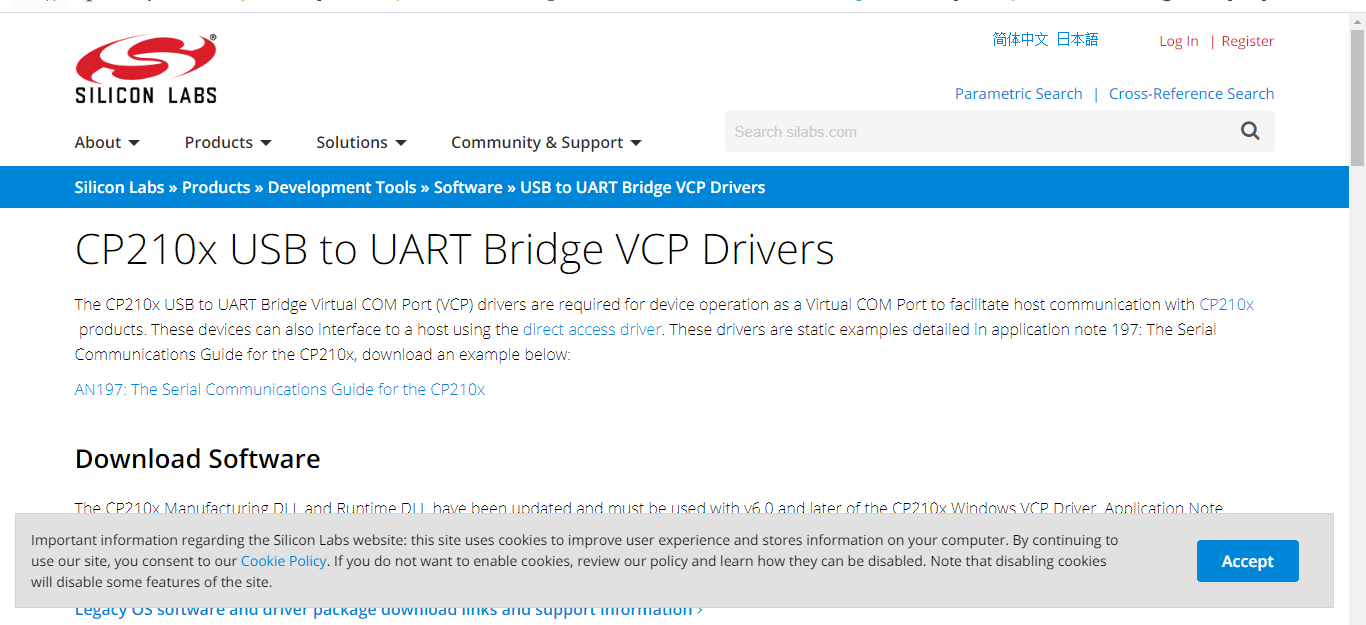
\includegraphics[width=1\textwidth]{figures/google3.png}
\caption{Tampilan Cp210 Driver }
\label{print}
\end{figure}
\par Setelah diklik Cp210 driver paling atas maka tampilan awal dari website tersebut seperti pada gambar.
\begin{figure}[H]
\centering
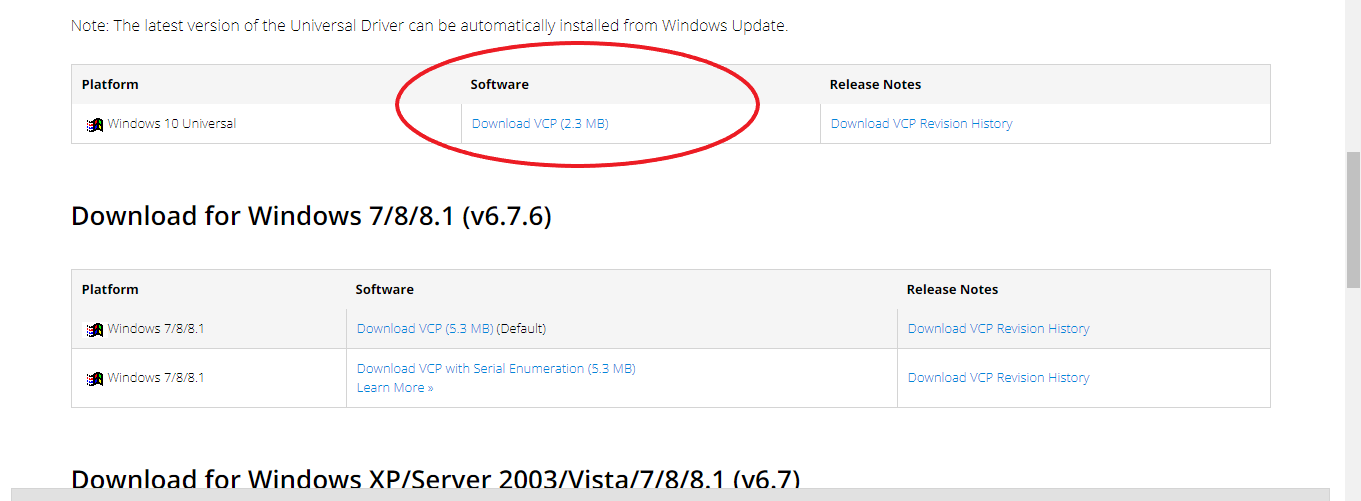
\includegraphics[width=1\textwidth]{figures/google4.png}
\caption{Tampilan Cp210 Driver Dwonload }
\label{print}
\end{figure}
\par Seteah masuk ke tampilan Cp210 scroll kebagian bawah sampai ada tulisan dwonload untuk window seperti gambar diatas. Kemudian pilih windows 10 jika menggunakan sistem operasi windows 10 jika tidak memakai maka harus disesuaikan.
\begin{figure}[H]
\centering
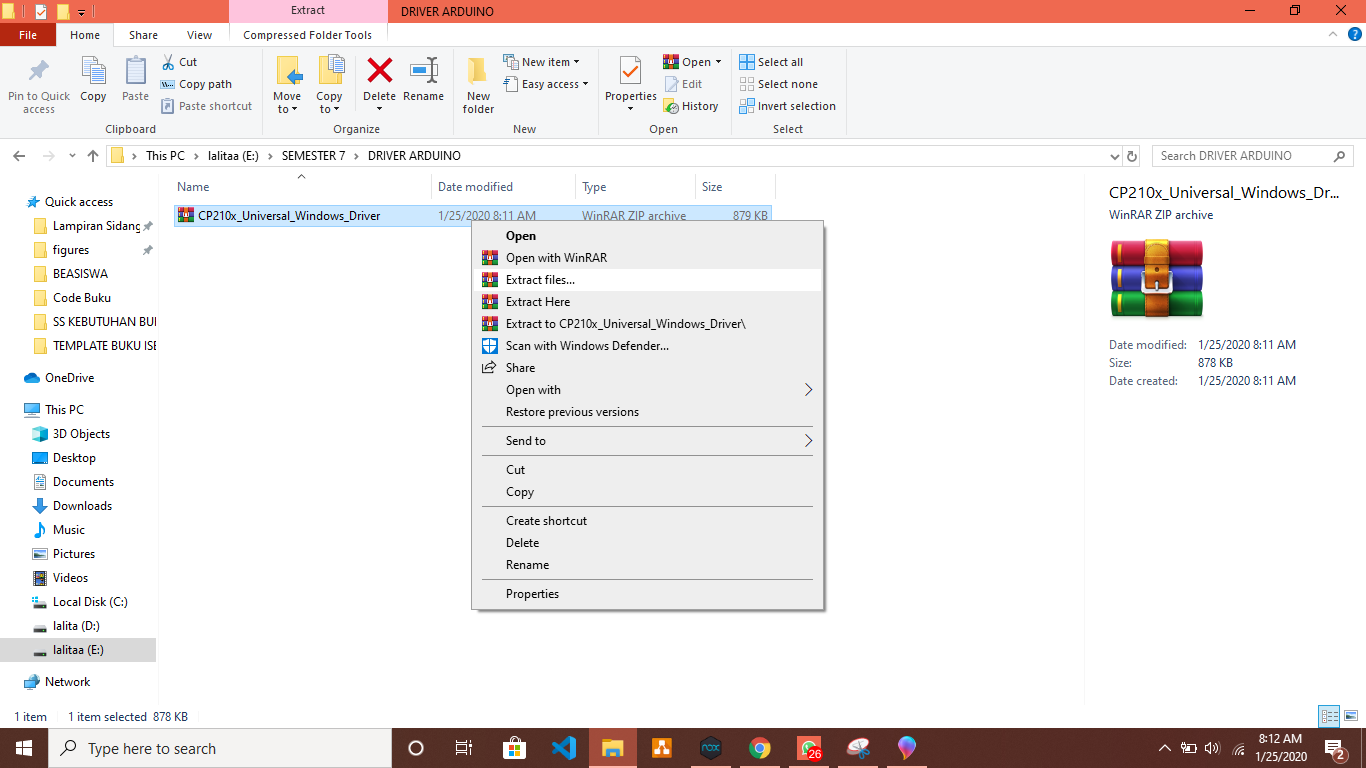
\includegraphics[width=1\textwidth]{figures/google5.png}
\caption{Tampilan Hasil Dwonload Driver }
\label{print}
\end{figure}
\par Setelah di \textit{dwonload} maka file yang didapatkan dari hasil \textit{dwonload} berupa Rar. Kemudian klik kanan dan pilih extract here.

\begin{figure}[H]
\centering
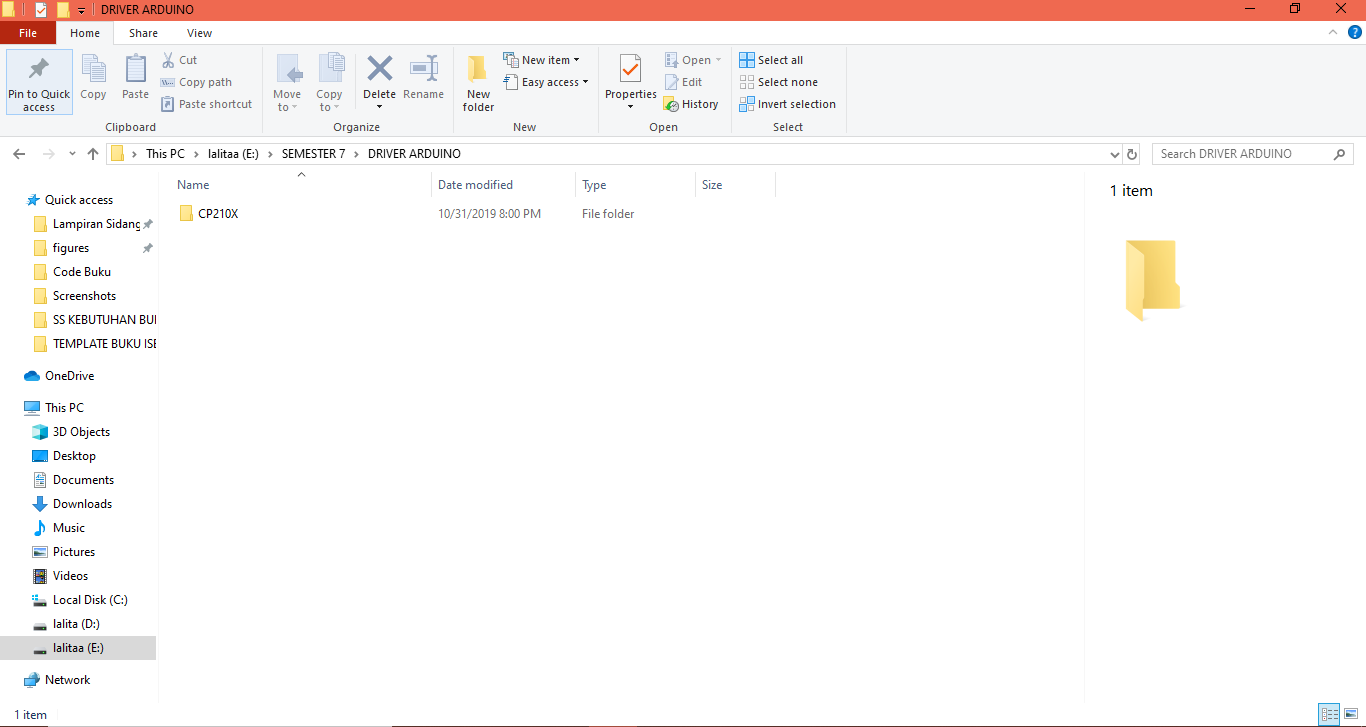
\includegraphics[width=1\textwidth]{figures/google6.png}
\caption{Tampilan File Hasil \textit{extract} }
\label{print}
\end{figure}
\par Hasil file yang sudah di extrac akan menjadi sebuah folder seperti pada gambar diatas.
\begin{figure}[H]
\centering
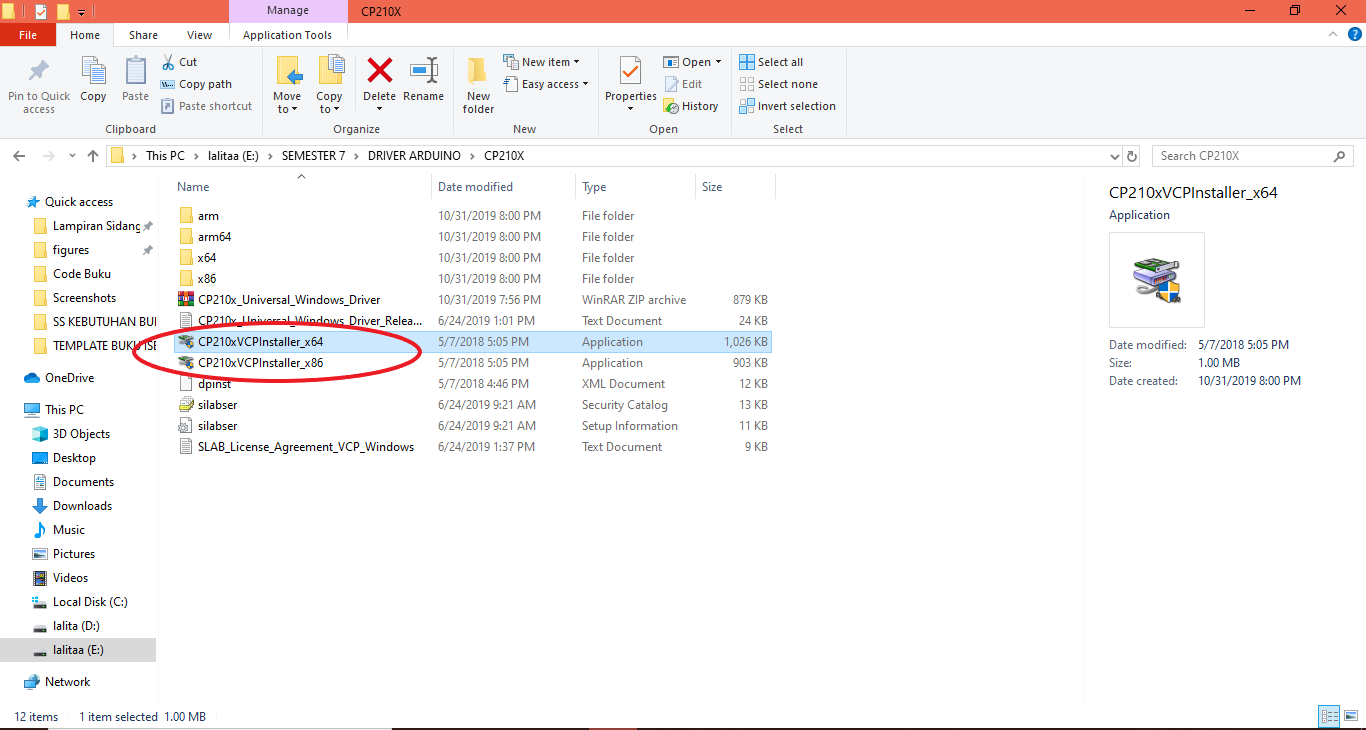
\includegraphics[width=1\textwidth]{figures/google7.png}
\caption{Tampilan File Cp210 Driver}
\label{print}
\end{figure}
\par Buka folder tersebut kemudian pilih CP210.exe seperti pada gambar diatas yang bertujuan untuk di \textit{installs}. Disini \textit{intstall} driver Cp210 64 byte dan apabila memkai yang 32 byte maka pilih file yang ujungnya x86. Kemudian  jika sudah menginstall driver Cp210 maka selanjutnya harus menginstall driver Ch340x seperti berikut.
\begin{figure}[H]
\centering
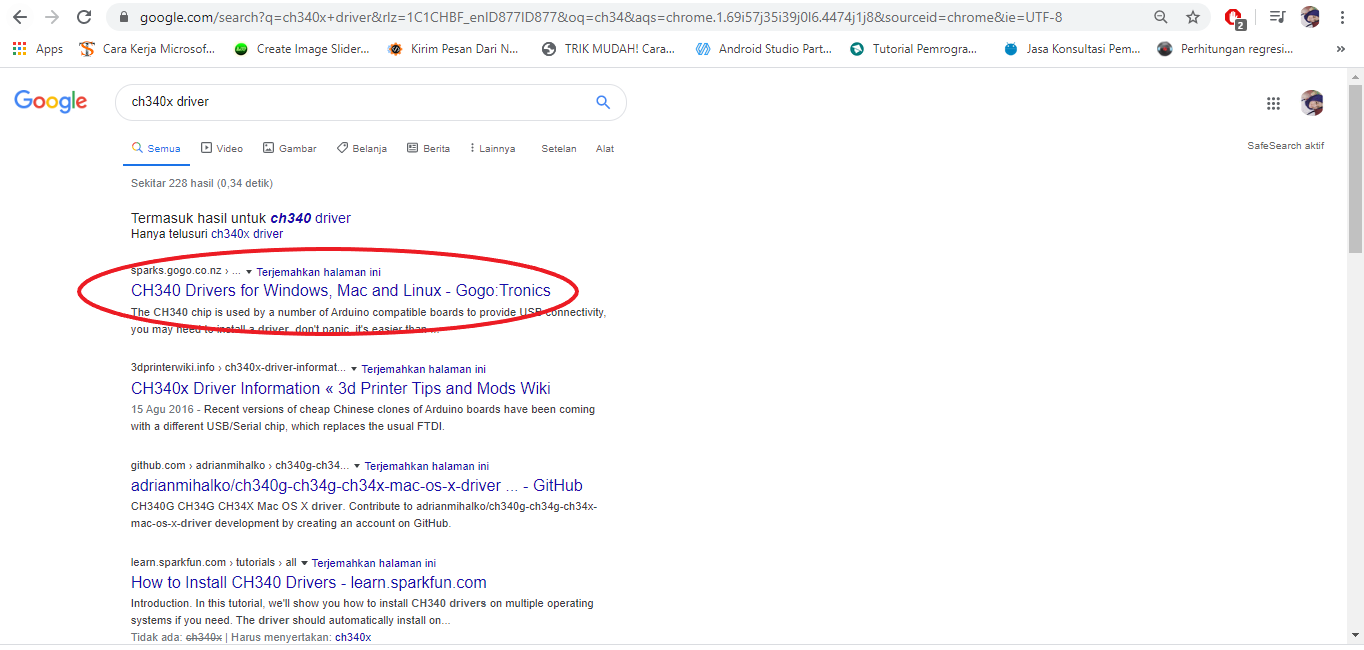
\includegraphics[width=1\textwidth]{figures/google8.png}
\caption{Tampilan Hasil Pencarian }
\label{print}
\end{figure}
\par Ketik atau mencari Ch340x driver di google.  maka Google akan menampilkan hasil pencari dari beberapa referensi. Kemudian klik hasil pencarian Ch340x driver paling atas seperti pada gambar diatas.
\begin{figure}[H]
\centering
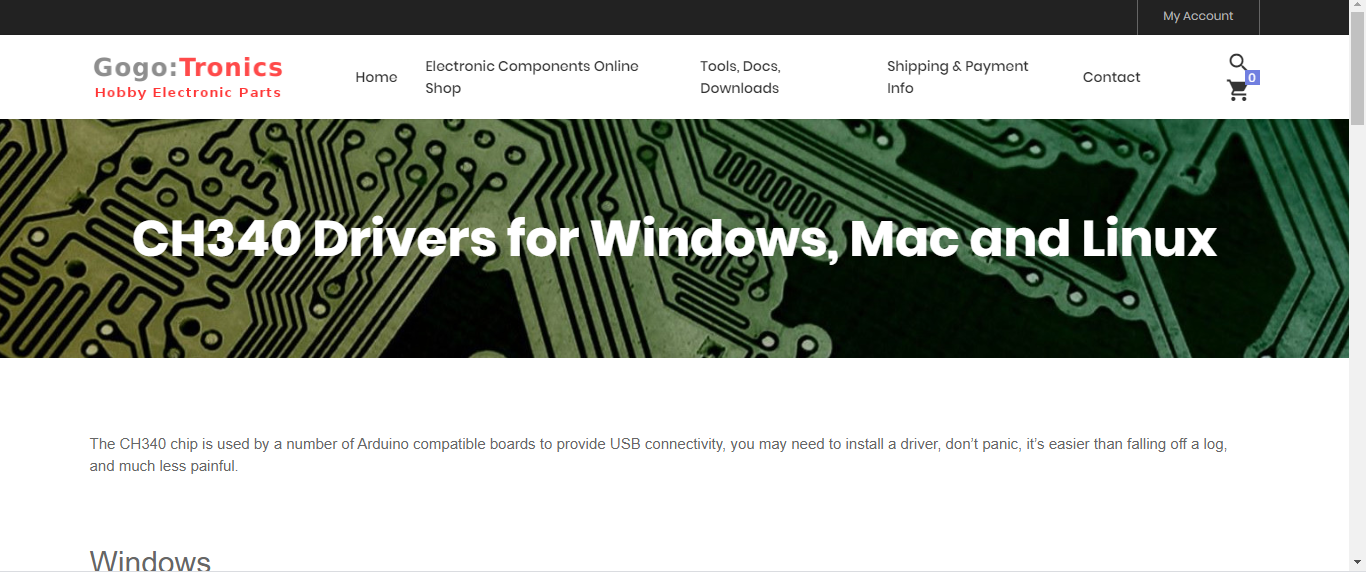
\includegraphics[width=1\textwidth]{figures/google9.png}
\caption{Tampilan Hasil Pencarian }
\label{print}
\end{figure}
\par Setelah diklik Ch340x driver paling atas maka tampilan awal dari website tersebut seperti pada gambar.
\begin{figure}[H]
\centering
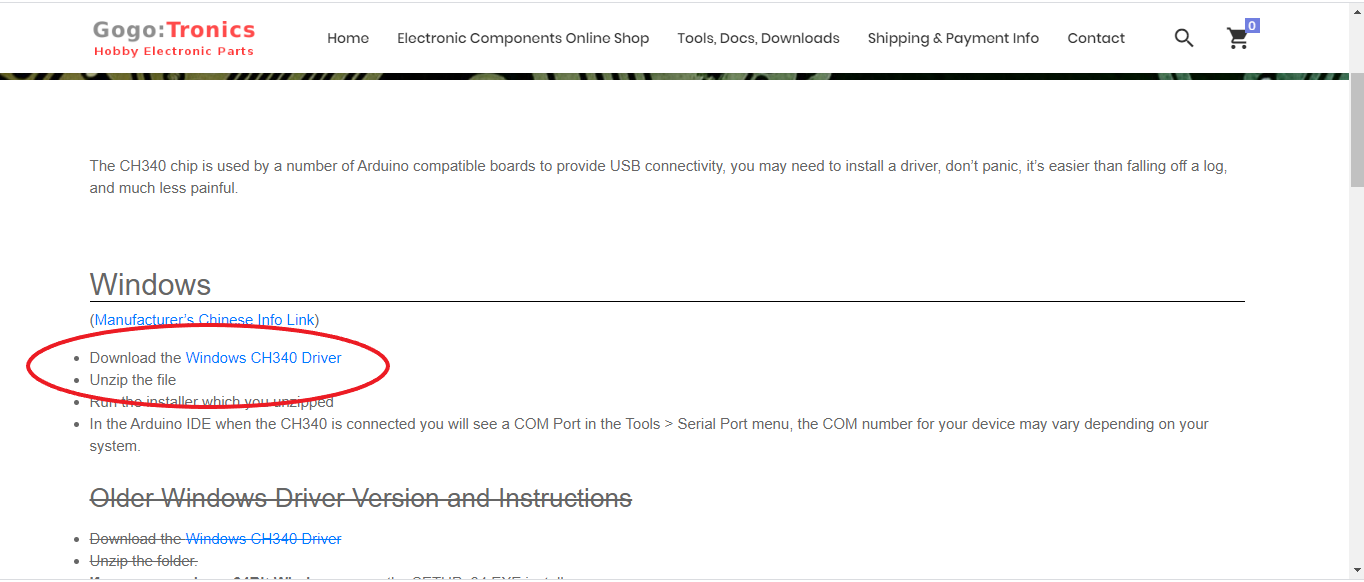
\includegraphics[width=1\textwidth]{figures/google10.png}
\caption{Tampilan Ch340x Driver Dwonload }
\label{print}
\end{figure}
\par Seteah masuk ke tampilan Ch340x scroll kebagian bawah sampai ada tulisan dwonload untuk window seperti gambar diatas. Kemudian pilih windows CH340 Driver.
\begin{figure}[H]
\centering
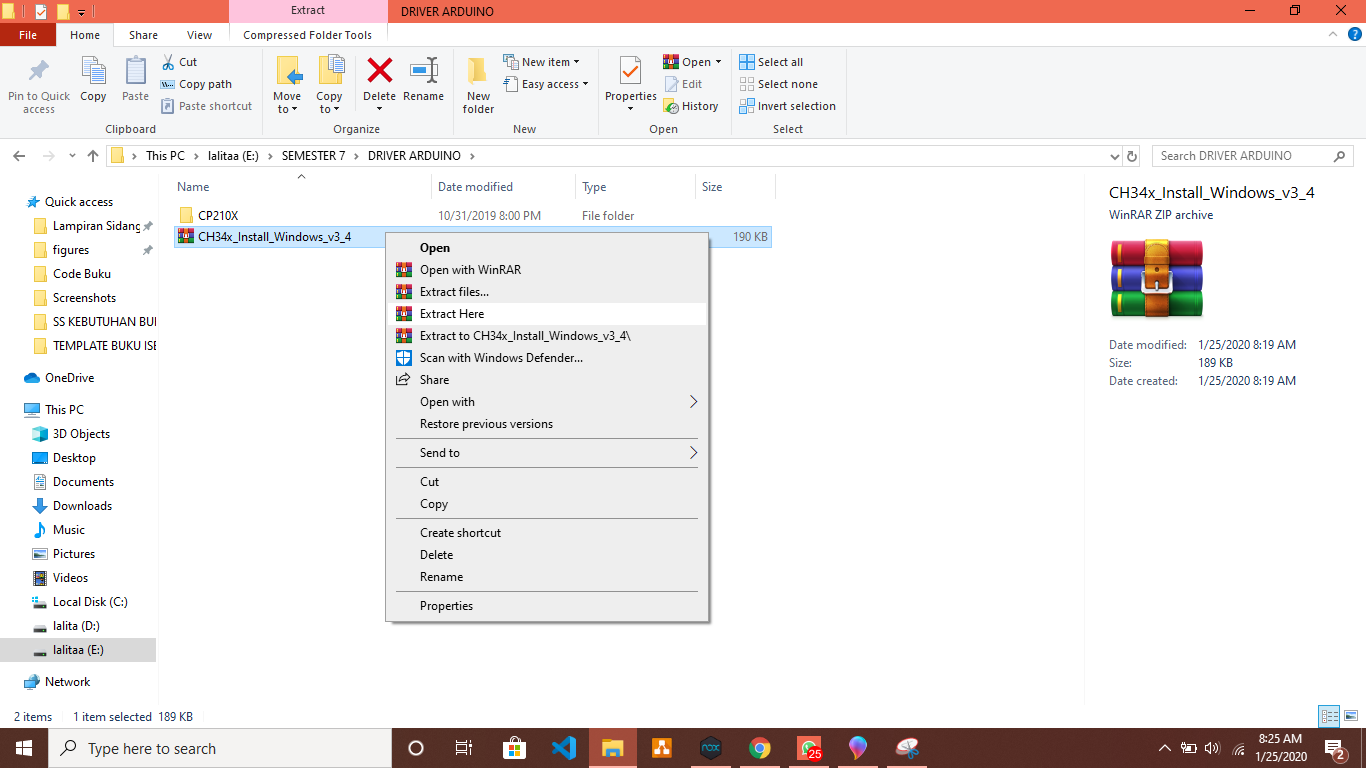
\includegraphics[width=1\textwidth]{figures/google11.png}
\caption{Tampilan Hasil Dwonload Driver }
\label{print}
\end{figure}
\par Setelah di \textit{dwonload} maka file yang didapatkan dari hasil \textit{dwonload} berupa Rar. Kemudian klik kanan dan pilih extract here.
\begin{figure}[H]
\centering
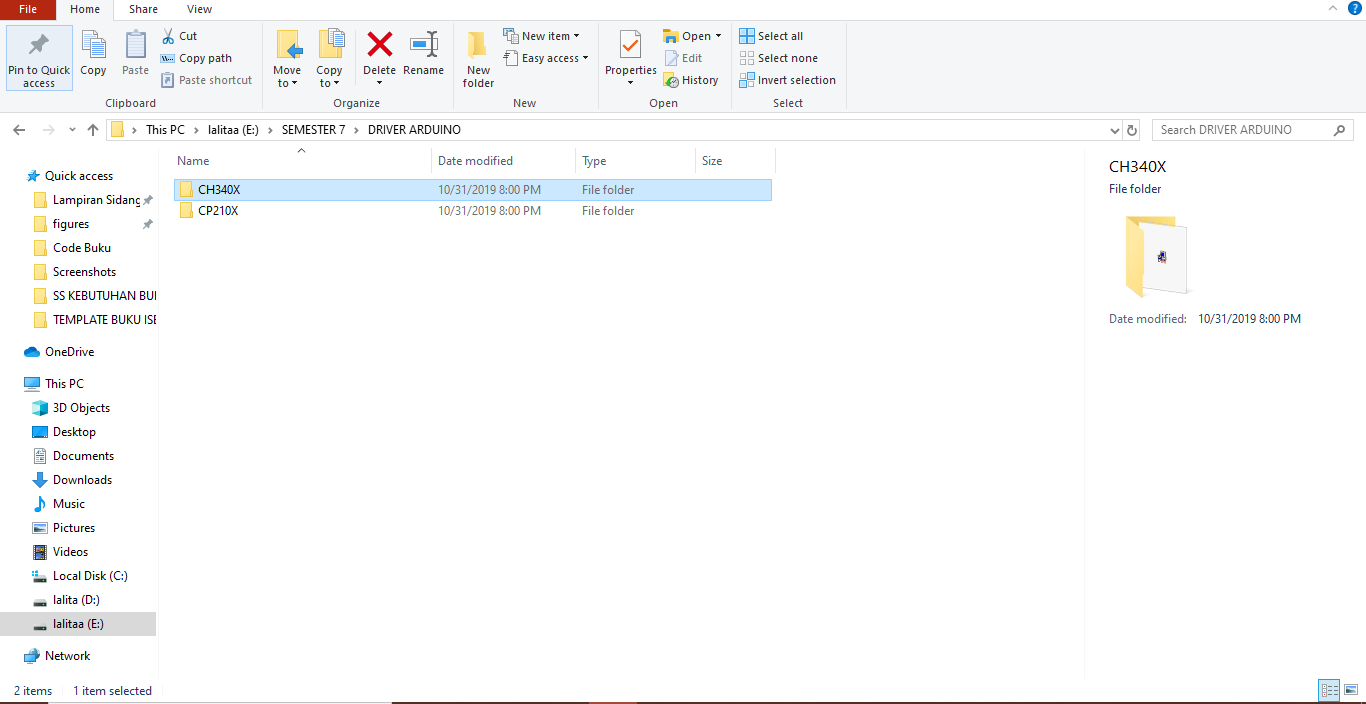
\includegraphics[width=1\textwidth]{figures/google12.png}
\caption{Tampilan File Hasil \textit{extract} }
\label{print}
\end{figure}
\par Hasil file yang sudah di extrac akan menjadi sebuah folder seperti pada gambar diatas.
\begin{figure}[H]
\centering
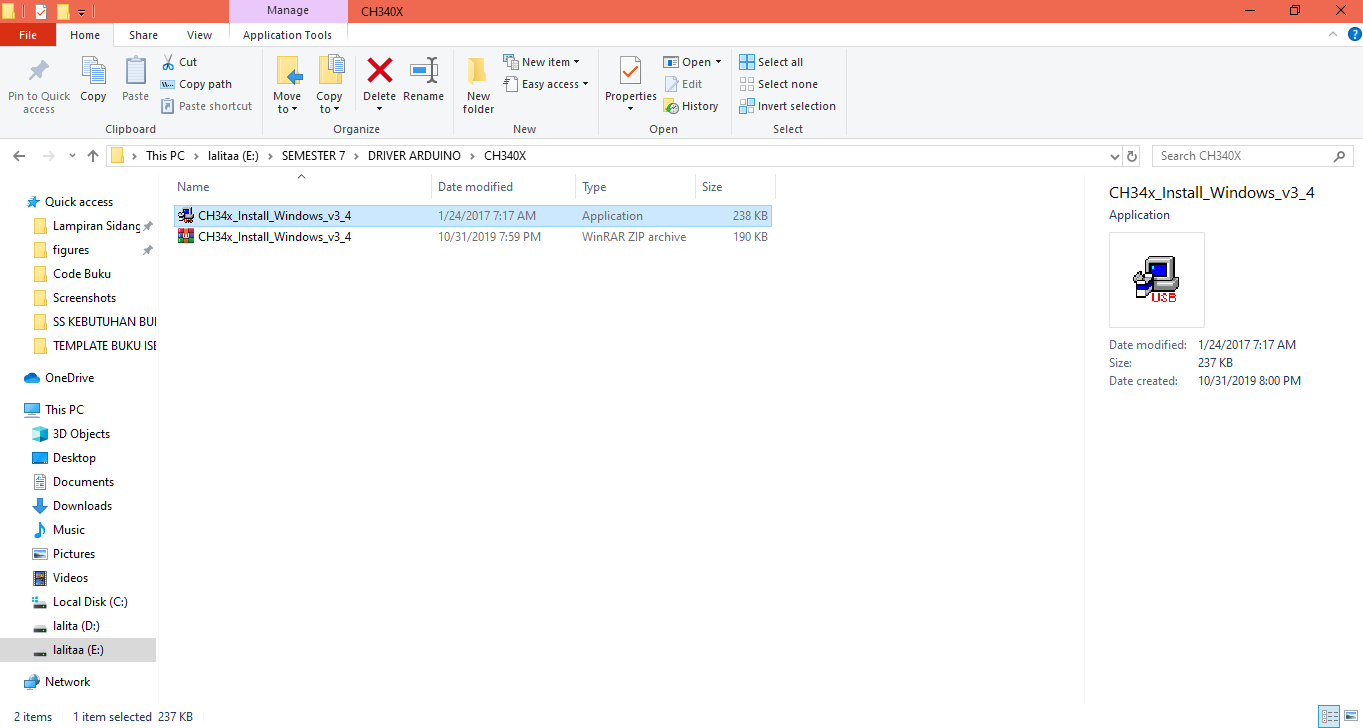
\includegraphics[width=0.5\textwidth]{figures/google13.png}
\caption{Tampilan File CH340x Driver}
\label{print}
\end{figure}
\par Buka folder tersebut kemudian pilih CH340x.exe seperti pada gambar diatas yang bertujuan untuk di \textit{installs}.Setelah kita selesai menginstall driver yang dibutuhkan maka tahapan selajutnya yaitu memprogram nodemcu di arduino IDE.


\subsection{Contoh Pemograman Di Arduino IDE}
Kini saatnya menjalankan Arduino IDE, pilih File > Examples > Basic > Blink  . Maka akan muncul pada jendela yang berisi source sebagai berikut:
\begin{figure}[H]
\centering
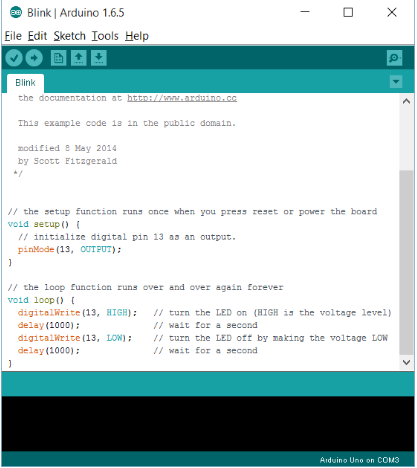
\includegraphics[width=0.7\textwidth]{figures/ide4.png}
\caption{Tampilan Arduino IDE Blink}
\label{print}
\end{figure}

\par Program ini memerintahkan Arduino untuk memberi sinyal digital bergantian dari  0 V dan 5V pada port 13. Kenapa Port 13? Karena di Port 13 Arduino Uno, terdapat  LED orange kecil yang tertanam dalam board sehingga untuk mengetes apakah arduino kita berfungsi atau tidak, cukup program port 13 untuk mengirimkan sinyal digital dan lihat hasilnya secara visual pada LED tersebut. Langkah selanjutnya perhatikan berikut ini :
\begin{enumerate}
    \item \textbf{Pilih Port Serial} 
    \par Sebelum kita mengupload program ke dalam board, pilih port usb dimana Arduino Uno terbaca. Pilih Tools > Port  untuk menyambungkan port.
    \item \textbf{\textit{Upload Program}}
    \par Setelah koneksi ke port serial sudah oke, klik tombol \textit{“Upload”} pada Arduino IDE. dan tunggu beberapa saat hingga muncul pesan \textit{“Done Uploading”} pada status bar. Jika berhasil, kita akan melihat LED orange arduino Uno akan berkedip-kedip dengan delay tertentu.
\par Setelah Blink kita akan membuat "Hello Word" menggunakan Arduino IDE yang nantinya akan di tampilkan di serial monitor. Berikut code pemogramannya :
\lstinputlisting{src/hello.c}
\par Setelah program diatas diketikkan pada software Arduino IDE, maka tahap selanjutnya lakukan proses \textit{Upload} kedalam board Arduinonya tunggu sampai proses selesai sampai ada tanda \textit{Done Uploading}. Untuk melihat hasilnya klik menu Tools kemudian Serial Monitor maka hasilnya akan muncul seperti gambar berikut.
\begin{figure}[H]
\centering
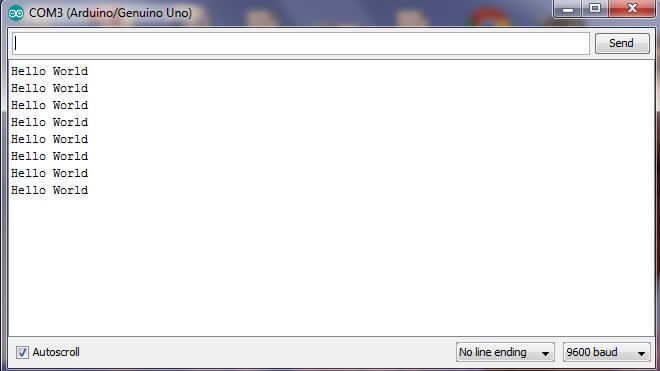
\includegraphics[width=1\textwidth]{figures/hello.jpg}
\caption{Tampilan Di Serial Monitor}
\label{print}
\end{figure}
\par Penjelasan tentang fungsi-fungsi dari tiap-tiap bagian program diatas adalah sebagai berikut:
\begin{enumerate}
    \item Void Setup()  adalah fungsi yang dijalankan secara otomatis pertama kali oleh board Arduino, dimana Semua kode program yang ada dalam void setup akan dibaca sekali oleh Arduino. Biasanya isinya berupa kode perintah untuk menentukan fungsi pada sebuah pin atau deklarasi INPUT/OUTPUT.
    \item “begin()” digunakan untuk mengatur baudrate / kecepatan transmisi data. Beberapa pilihan kecepatan komunikasi data yang dapat digunakan pada board arduino adalah 300, 1200, 2400, 4800, 9600, 14400, 19200, 28800, 38400, 57600 atau 115200. Pengaturan baudrate dilakukan pada bagian setup().
    \item Void loop() melakukan proses dimana semua kode yang ada disini akan dibaca berulang kali (terus menerus) oleh Arduino.
    \item Perintah “Serial.print” digunakan untuk menampilkan data ke serial monitor. Data yang ditampilkan dapat berupa karakter, bytes, atau angka.
    \item delay(2000) merupakan pernyataan untuk melakukan penundaan selama 2000 milidetik atau 2 detik dari proses akhir pembacaan program sebelumnya dimana Arduino akan mengulang proses pembacaan program dari awal kembali.
\end{enumerate}
\end{enumerate}
\subsection{Cara \textit{Import Library}}
\par Library adalah kumpulan code yang biasanya terkumpul dalam sebuah namespace/ module/ package (tergantung anda menggunakannya di bahasa pemrograman apa) yang dapat di import/ reuse ke program lain. Untuk mengimport library ada tiga cara yaitu menggunakan \textit{manager library}, mengimport library .zip hasil dwonload dan Instalasi Manual.
\begin{enumerate}
    \item Import Library Menggunakan Manager
\par Untuk menginstal sebuah Library baru ke dalam IDE Arduino,dapat menggunakan Library Manager (tersedia sejak Arduino IDE versi 1.6.2). Buka Arduino IDE dan klik ke menu “Sketch” dan kemudian Include Libary > Manage Libraries .
\begin{figure}[H]
\centering
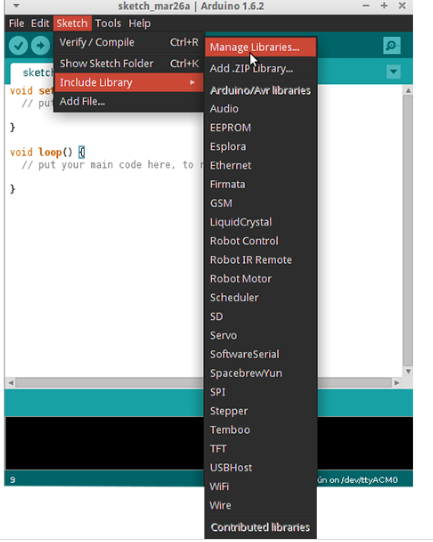
\includegraphics[width=0.7\textwidth]{figures/manager1.png}
\caption{Memilih Menu Manage Librarie}
\label{print}
\end{figure}

\par Kemudian Sketch Manager akan terbuka dan  akan menemukan daftar Library yang sudah terpasang ataupun Library baru yang siap untuk di instalasi. Dalam contoh ini kita akan menginstal library Bridge. Gulir daftar untuk menemukannya, lalu pilih versi Library yang ingin Anda instal. (beberapa Library terkadang hanya ada satu versi Library yang tersedia).
\begin{figure}[H]
\centering
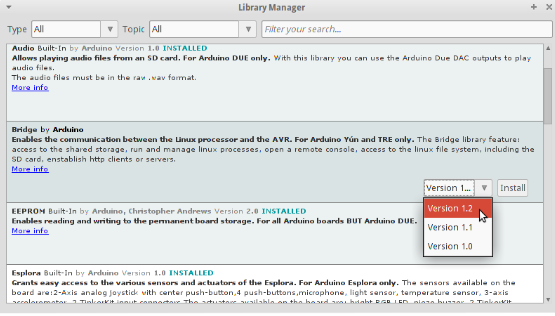
\includegraphics[width=0.9\textwidth]{figures/manager2.png}
\caption{Tampilan Sketch Manager}
\label{print}
\end{figure}
\par Langkah selanjtnya adalah klik instal dan tunggu IDE untuk menginstal library baru. Setelah selesai, sebuah tag Installed akan muncul di sebelah Library Bridge.  Setelah terinstal, sekarang kita dapat menemukan Library baru yang tersedia di menu Include Library.
\begin{figure}[H]
\centering
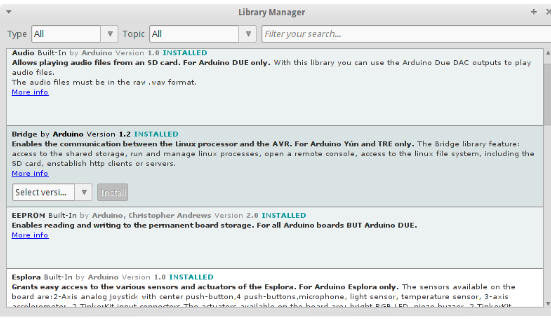
\includegraphics[width=0.9\textwidth]{figures/manager3.png}
\caption{Tampilan Library Yang Terinstall}
\label{print}
\end{figure}

\item  Mengimport Libray .zip hasil Download.

\par Terkadang Library hasil buatan sesorang banyak dan sering yang didistribusikan sebagai file ZIP atau folder sehingga dapat kita unduh, di GitHub misalnya. Nama folder adalah nama Library. Di dalam folder tersebut akan ada file .cpp, file .h , Folder Contoh Sketch, dan file lainnya yang dibutuhkan oleh Library. Dimulai dengan versi 1.0.5, Kita bisa menginstal library pihak ke-3 di IDE. Jangan unzip Libray yang telah didownload, biarkan seperti apa adanya.

\par Buka aplikasi Arduinonya, lalu Masuk ke menu SKETCH, pilih INCLUDE LIBRARY, pilih ADD. ZIP Library , seperti gambar berikut :
\begin{figure}[H]
\centering
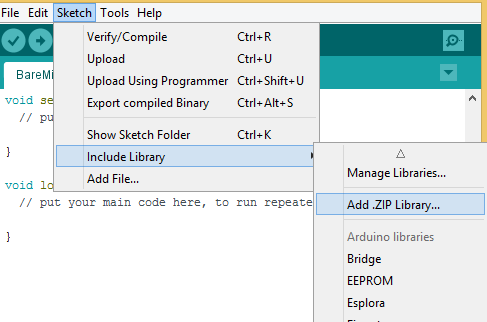
\includegraphics[width=0.7\textwidth]{figures/library1.png}
\caption{Tampilan Library ADD ZIP}
\label{print}
\end{figure}

\par Kemudian  akan diminta untuk memilih Library yang ingin ditambahkan. klik add .ZIP library, lalu cari file ZIP yang sudah didwonload.
\begin{figure}[H]
\centering
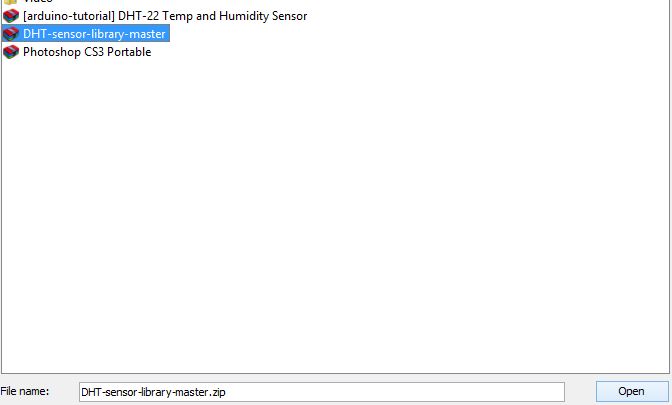
\includegraphics[width=0.9\textwidth]{figures/library2.png}
\caption{Pilih File ZIP}
\label{print}
\end{figure}

\par  Jika berhasil, aplikasi Arduino kamu akan muncul keterangan seperti dibawah ini:
\begin{figure}[H]
\centering
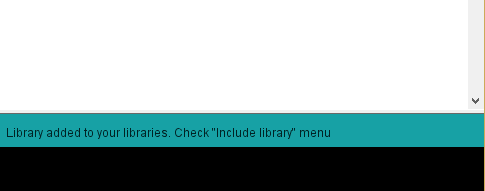
\includegraphics[width=0.9\textwidth]{figures/library3.png}
\caption{Tampilan Library Berhasil Ditambahkan}
\label{print}
\end{figure}

\item Instalasi Manual

\par Bila ingin menambahkan Library secara manual,  perlu mendownload sebagai file ZIP, lalu extrack file tersebut. (Klik Kanan pada File ZIP lalu pilih extract to “nama file” ), setelah folder hasil extrakan tersedia, selanjutnya kita harus memasukannya kedalam folder di C:User-NamaPC-Documents-Arduino-libraries.
\end{enumerate}

\section{Memprogram Komponen \textit{Prorotype PKA}}
\par Setalah kita mengetahui cara penggunaan Arduino IDE,\textit{import library}, dan struktur pemogramannya yang telah dibahas sebelum nya maka, tahapan selanjutnya yaitu mempogram komponen untuk \textit{prototype} PKA ini. Dengan cara memprogram serta testing komponen satu persatu kemudian digabungkan menjadi kesatuan yang utuh.
\subsection{Memprogram Sensor Ultasonic}
\par komponen pertama yang akan di program atau di tes yaitu sensor ultrasonic US 100 yang nantinya berfungsi untuk membaca jarak ketinggian air. Berikut kodinganya :
\lstinputlisting{src/sensor.c}
\par Penjelasan coding diatas yaitu :
\begin{enumerate}
    \item #define triggerPin  D4 #define echoPin D3
\par Script tersebut untuk menginsiasi pin yang akan digunakan. Pin D4 digunakan untuk pin trigger dan D3 digunakan untuk pin echo.
\item Serial.begin (9600); ,pinMode(triggerPin, OUTPUT); ,pinMode(echoPin, INPUT); 
\par Script diatas berada di fungsi void setup(). Serial.begin() digunakan untuk memulai serial. selanjutnya pinMode digunakan untuk menentukan fungsi dari pin yang akan digunakan (triggerPin dan echoPin). triggerPin berfungsi sebagai pin output sedangkan echoPin sebagai pin input.
\item long duration, jarak;
\par Script diatas digunakan untuk deklarasi variabel duration dan jarak. Duration dan jarak merupakan variabel bertipe long. Long merupakan tipe data serupa dengan int tetapi memiliki range yang lebih panjang.
\item   digitalWrite(triggerPin, LOW);,  delayMicroseconds(2);,  digitalWrite(triggerPin, HIGH);,  delayMicroseconds(10);  digitalWrite(triggerPin, LOW);
\par Script tersebut menjelaskan bahwa pin trigger menembakkan pulsa sinyal ultrasonik selama 10 micro second.
\item duration = pulseIn(echoPin, HIGH);
\par Selanjutnya ketika gelombang ultrasonik itu ditangkap kembali setiap pulsanya oleh pin echo maka waktu tangkap tersebut diubah menjadi variabel duration.
\item jarak = (duration/2) / 29.1;
\par Dengan persamaan diatas nilai waktu duration akan dikonversi menjadi nilai jarak dalam bentuk cm.
\item Serial.println("jarak :");,
  Serial.print(jarak);,
  Serial.println(" cm");,
  delay(1000);
\par Selanjutnya nilai jarak yang didapatkan akan ditampilkan di serial monitor setiap 1 detik (delay(1000)).

\end{enumerate}
\par Untuk melihat hasil pembacaan sensor lewat serial monitor pada arduino IDE. Jika sukses maka akan seperti gambar berikut :
\begin{figure}[H]
\centering
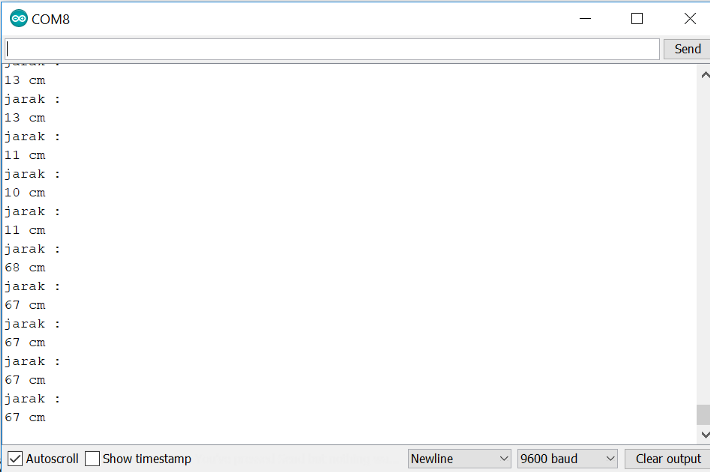
\includegraphics[width=0.9\textwidth]{figures/hasilsensor.png}
\caption{Tampilan serial monitor}
\label{print}
\end{figure}

\subsection{Memprogram Led}
\par Komponen kedua yang akan di program atau di tes yaitu led yang nantinya  berfungsi untuk sebagai indikator.Berikut Kodingannya :
\lstinputlisting{src/led.c}
\par Penjelasan coding diatas yaitu :
\begin{enumerate}
    \item const int ledPin = D2;
    \par Script tersebut untuk menginsiasi pin yang akan digunakan.
    \item pinMode(2, OUTPUT); 
    \par Menetapkan pin GPIO 2/LED sebagai OUTPUT.
    \item digitalWrite(2, LOW);
    \par  Perintah untuk mematikan Lampu atau memberikan nilai LOW(0) pada pin GPIO 2.
    \item delay(1000); 
    \par Matikan lampu selama 1 detik.
    \item digitalWrite(2, HIGH);
    \par Perintah memberikan nilai HIGH atau menyalakan Lampu.
    \item delay(2000);
    \par Nyalakan lampu selama 2 detik.
\end{enumerate}
\subsection{Memprogram Buzzer}
\par Komponen ketiga yang akan di program atau di tes yaitu buzzer yang nantinya  berfungsi untuk sebagai indikator.Berikut Kodingannya :
\lstinputlisting{src/buzzer.c}
\par Penjelasan coding diatas yaitu :
\begin{enumerate}
    \item const int ledPin = D1;
    \par Script tersebut untuk menginsiasi pin yang akan digunakan.
    \item pinMode(1, OUTPUT); 
    \par Menetapkan pin GPIO 1/Buzzer sebagai OUTPUT.
    \item digitalWrite(2, LOW);
    \par  Perintah untuk mematikan Buzzer atau memberikan nilai LOW(0) pada pin GPIO 1.
    \item delay(1000); 
    \par Matikan buzzer selama 1 detik.
    \item digitalWrite(1, HIGH);
    \par Perintah memberikan nilai HIGH atau menyalakan buzzer.
    \item delay(2000);
    \par Nyalakan buzzer selama 2 detik.
\end{enumerate}

\subsection{Memprogram Sensor, Led dan Buzzer}
\par Setelah memprogram komponen satu persatu maka selanjutnya menggabungkan komponen yang telah diprogram sebelumnya. Komponen yang akan digabungkan yaitu sensor, led , buzzer terlebih dahulu. Mengapa kita harus memprogram satu persatu terlebih dahulu tidak langsung ? alasan terlebih dahulu memprogram komponen satu persatu yaitu jika adanya error pada saat prosses penggabungan komponen akan mengetahui komponen manakah yang error. Berikut codingan dari komponen yang digabungkan :
\lstinputlisting{src/gabung.c}
\par Penjelasan coding diatas yaitu :
\begin{enumerate}
\item const int trigPin = 2;  //D4 ,
const int echoPin = 0;  //D3 ,
const int ledPin = 4;  //D2, 
const int buzzerPin = 5;  //D1
\par Script tersebut untuk menginsiasi pin yang akan digunakan. Pin D4 digunakan untuk pin trigger,D3 digunakan untuk pin echo, D2 digunakan untuk ledppin, dan D1 digunakan untuk buzzerpin.

\item // defines variables ,
long duration; ,
int distance;, 
int safetyDistance;
\par Script diatas merupakan sebuah pendefinisian variabel.
\item pinMode(trigPin, OUTPUT);,
pinMode(echoPin, INPUT); ,
pinMode(buzzerPin, OUTPUT); ,
pinMode(ledPin, OUTPUT);,
Serial.begin(115200); 
\par Pada script tersebut merupakan sebuah bagian void setup yang berfungsi sebagai output dan input dari komponen. Selain itu pada script tersebut adanya baudrate yang digunakan 115200 yang berfungsi untuk komunisai serial.

\item digitalWrite(trigPin, LOW); ,
delayMicroseconds(2);

\par Script diatas merupakan sebuah perintah untuk mematikan (\textit{Low} pada trigpin disensor ultrasonic.

\item digitalWrite(trigPin, HIGH ,
delayMicroseconds(10); ,
digitalWrite(trigPin, LOW);
 
 \par Pada bagian script diatas merupakan sebuah perintah untuk trigpin pada sensor ultrasonic dan akan adanya jeda sebesar 10 detik.
 
 \item safetyDistance = distance;//
if (safetyDistance <= 5){//
  digitalWrite(buzzerPin, HIGH);//
  digitalWrite(ledPin, HIGH);//
}//
else{//
  digitalWrite(buzzerPin, LOW);//
  digitalWrite(ledPin, LOW);//
}
\par Script tersebut merupakan sebuah logika dari sensor ultrasonic. Dimana jika jarak yang dibaca oleh sensor ultrasonic adalah kurang dari sama dengan 5  maka buuer dan led akan menyala dan jika tidak membaca jarak kurang sama dengan 5 buzzr dan led mati.

\item Serial.print("Distance: "); ,
Serial.println(distance); ,
Serial.print("pulseIn "); ,
Serial.print("duration "); ,

\par Bagian script tersebut merupakan sebuah komunkasi serial yang nantinya jarak yang dibaca oleh sensor akan di tampilkan di serial monitor.
\end{enumerate}
\subsection{Memprogram Komponen dan Antares}
Setelah semua komponen yang digabungkan sudah diprogram maka tahapan selanjutnya yaitu menambahkan pemograman untuk antaresnya. Antares tersebut akan digunakan sebagai media penyimpan data yang dibaca oleh sensor ultrasonic. Sebelum memprogram ada langkah-langkah yang harus dilakukan untuk tahapan antares ini yaitu :
\begin{enumerate}
    \item Registrasi di Antares menggunakan gmail. Untuk membuka halaman antares cukup ketikan https://antares.id/id/index.html pada browser maka akan muncul tampilan seperti gambar berikut.
    \begin{figure}[H]
    \centering
    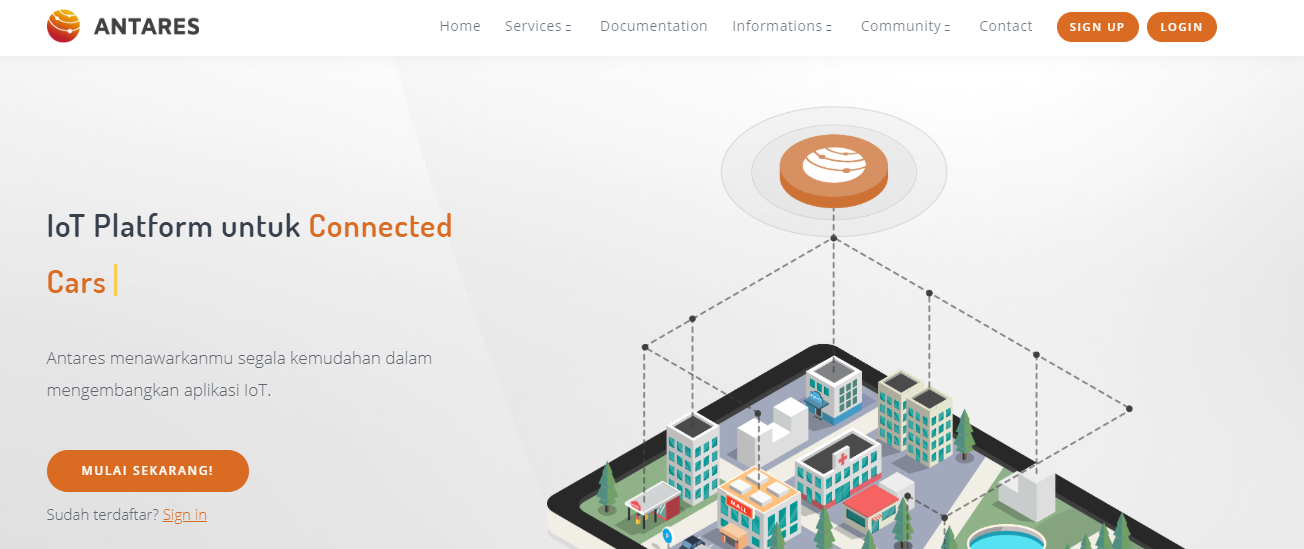
\includegraphics[width=1\textwidth]{figures/antares2.png}
    \caption{Halaman Awal Antares}
    \label{print}
    \end{figure}
    \par Setelah halaman tersebut muncul, pilih \textit{Signup} kemudian masukan email yang aktif.
    \begin{figure}[H]
    \centering
    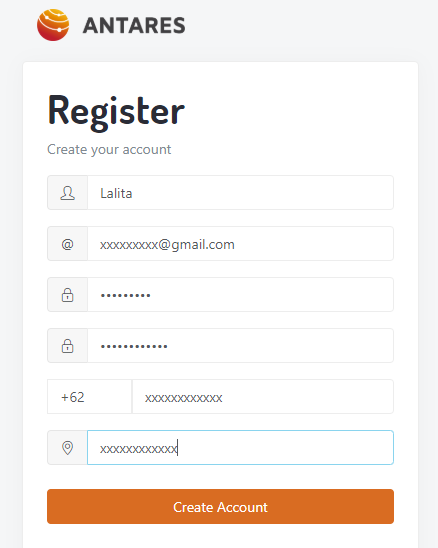
\includegraphics[width=1\textwidth]{figures/antares3.png}
    \caption{Tampilan Registrasi Antares}
    \label{print}
    \end{figure}
    \par Masukan nama , alamat email (alamat email aktif), password, no telepon dan alamat. Alamat email harus aktif karena ini berguna untuk \textit{verifikasi account} dan apabila ada info mengenai antares akan dikirmkan melalui email. 
    
    \begin{figure}[H]
    \centering
    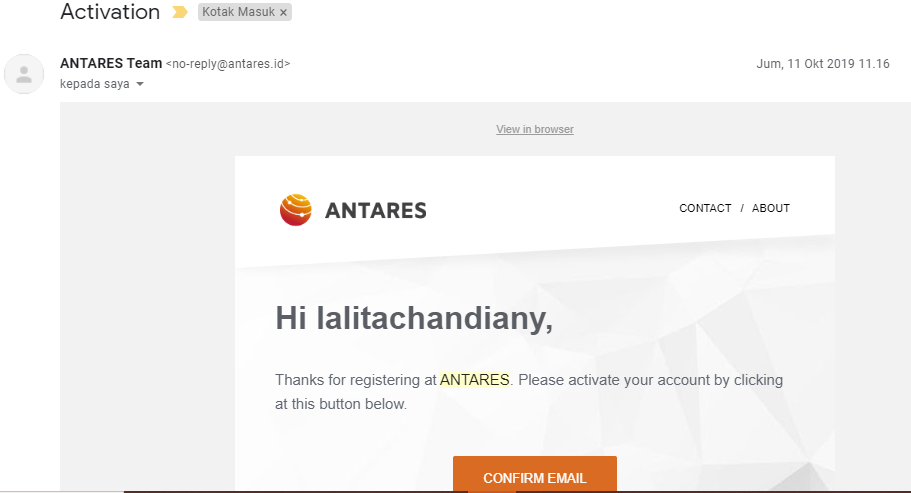
\includegraphics[width=1\textwidth]{figures/antares4.png}
    \caption{Verifikasi email}
    \label{print}
    \end{figure}
    
    \par Setelah melakukan registrasi di antares maka akan adanya email \textit{verifikasi} pada email yang sebelumnya email tersebut di daftarkan. Untuk mengkonfirmasi \textit{verifikasi} dari pihak antares cukup klik \textit{confirm}
    \begin{figure}[H]
    \centering
    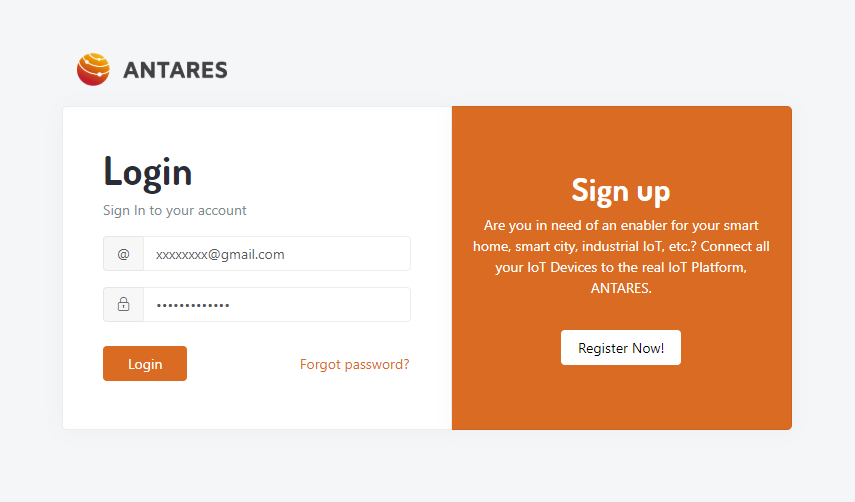
\includegraphics[width=1\textwidth]{figures/antares5.png}
    \caption{Login Antares}
    \label{print}
    \end{figure}
    \par setelah kita meng\textit{confirm} antares di email maka kita harus login di antares dengan mamasukan email yang telah didaftarkan dan memasukan password yang sebelumnya telah dibuat.
    
    \begin{figure}[H]
    \centering
    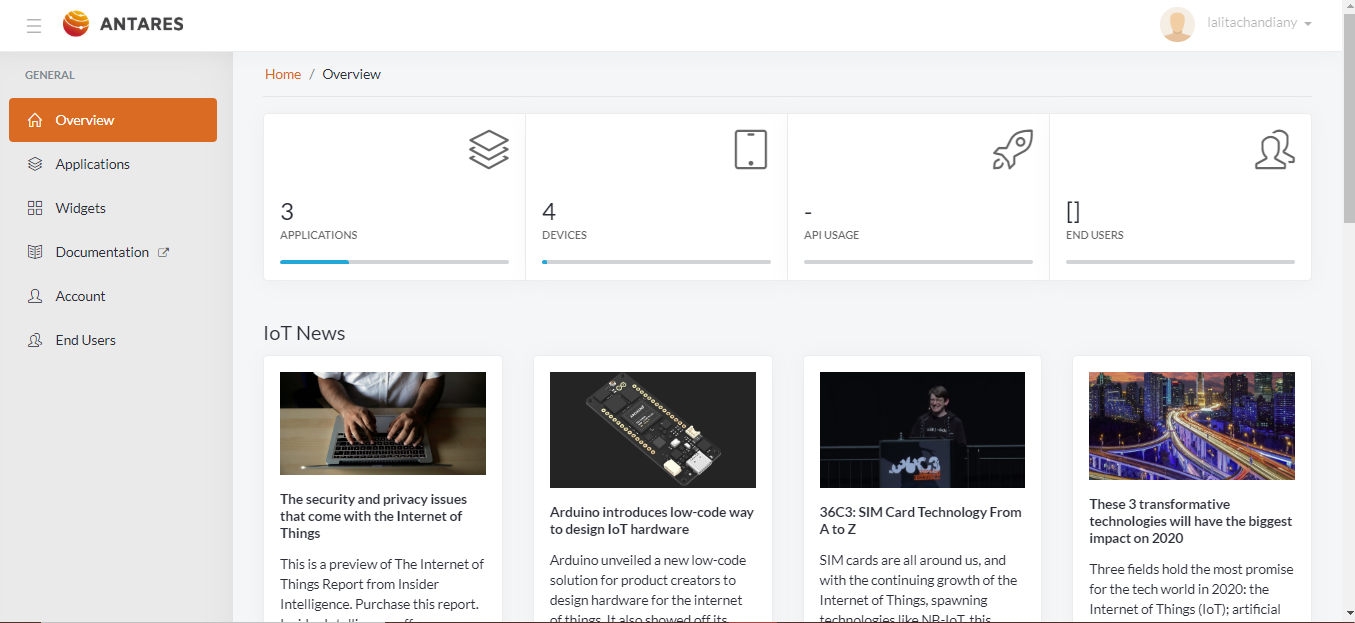
\includegraphics[width=1\textwidth]{figures/antares6.png}
    \caption{Tampilan Awal Antares}
    \label{print}
    \end{figure}
    
    \par Gambar diatas merupakan halaman awal antares ketika kita sudah login. Dalam halaman ini adanya beberapa menu yaitu :
    \begin{enumerate}
        \item \textit{Overview}
        \item \textit{Application}
        \item \textit{Widgets}
        \item \textit{Documentation}
        \item \textit{Account}
        \item \textit{Enduser}
    \end{enumerate}
     \begin{figure}[H]
    \centering
    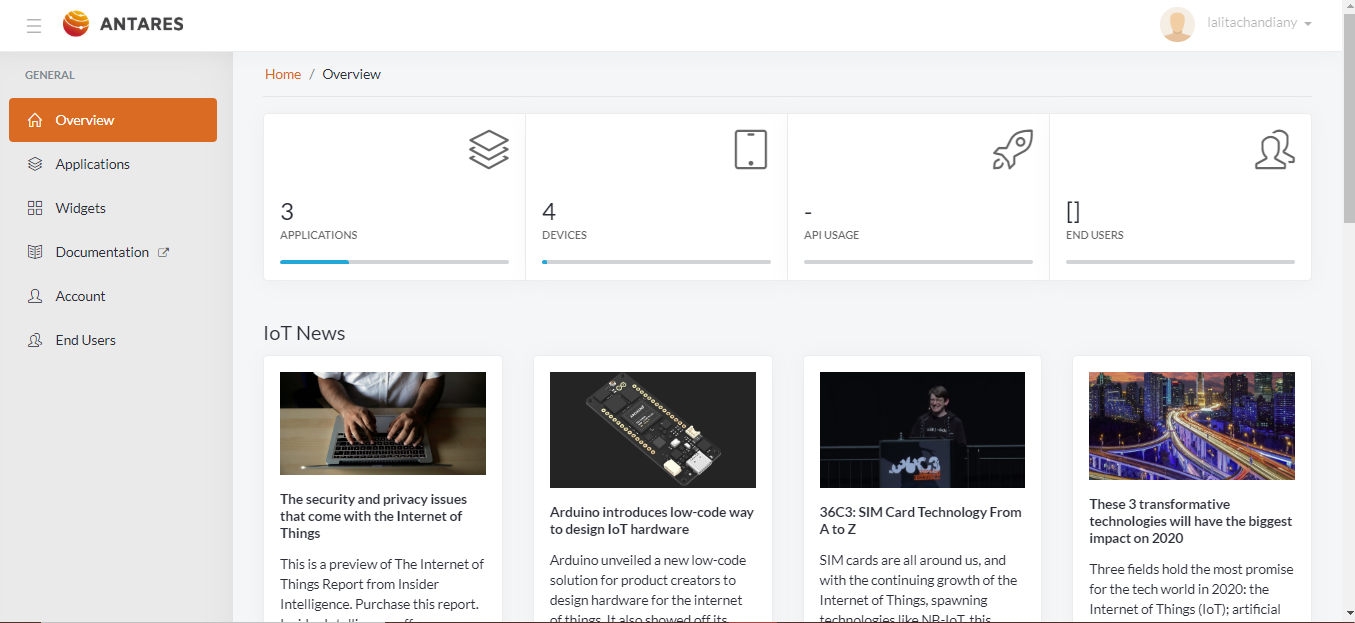
\includegraphics[width=1\textwidth]{figures/antares6.png}
    \caption{Halaman \textit{Overview}}
    \label{print}
    \end{figure}
    \par Halaman \textit{Overview} merupakan halaman awal yang ditampilkan pada saat setelah login. Halaman ini menampilkan sebuah berita mengenai IoT (\textit{Internet of Thing)}. Selain mengenai berita IoT halaman ini juga menampikan project yang sudah kita buat. Adanya \textit{application, device, API useage dan enduser.}
    \begin{figure}[H]
    \centering
    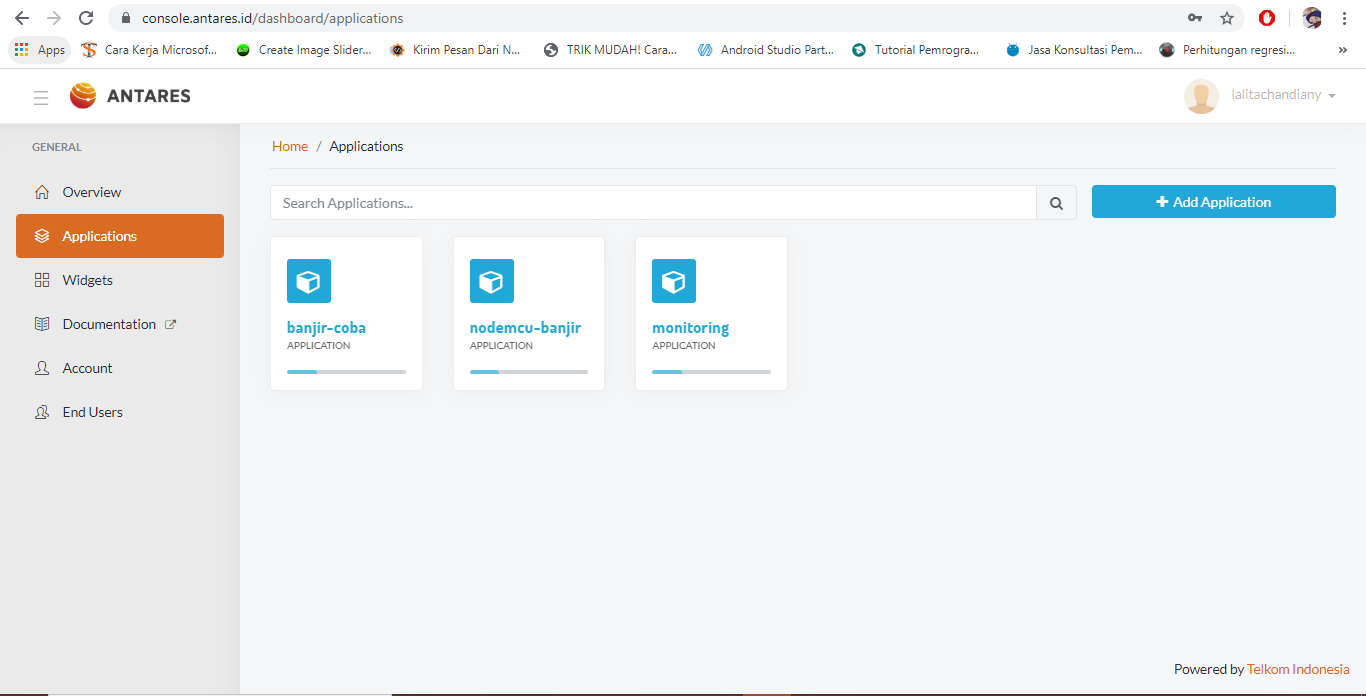
\includegraphics[width=1\textwidth]{figures/antares7.png}
    \caption{Halaman \textit{Apllication}}
    \label{print}
    \end{figure}
    \par Pada halaman \textit{application} menapilkan \textit{project} yang telah dibuat. Kemudian pada halaman ini kita dapat membuat sebuah project baru.
      \begin{figure}[H]
    \centering
    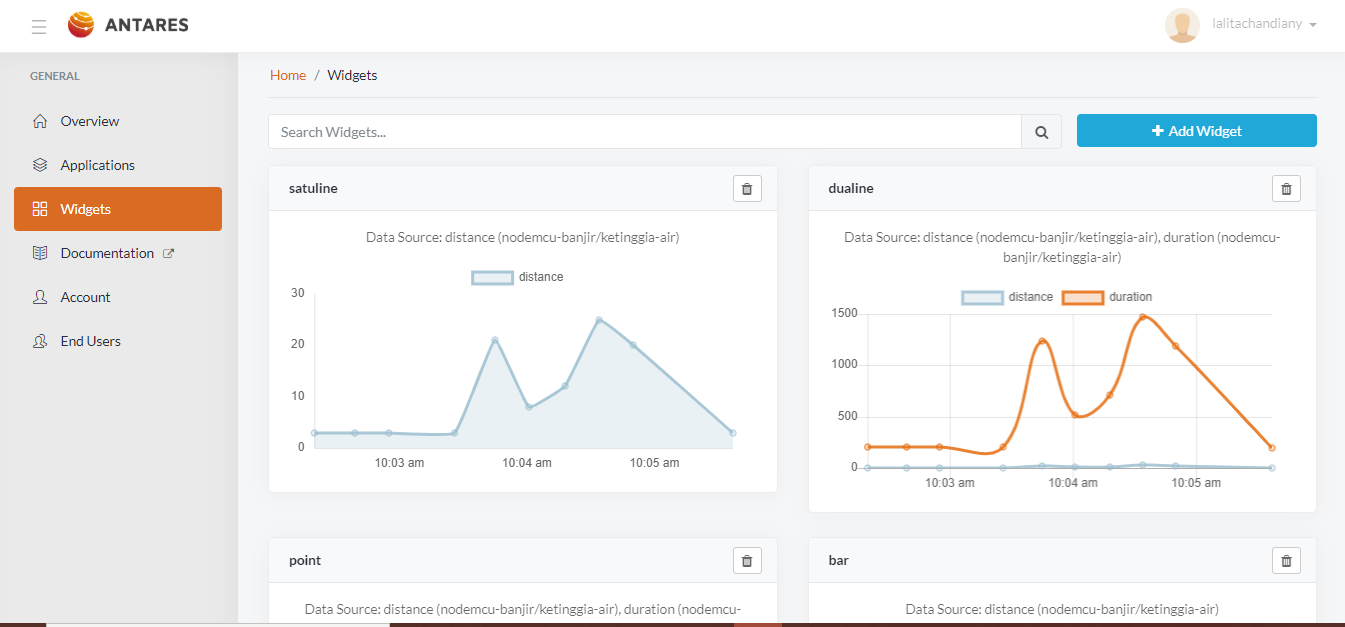
\includegraphics[width=1\textwidth]{figures/antares8.png}
    \caption{Halaman \textit{Widgets}}
    \label{print}
    \end{figure}
    
    \par Halaman widget merupakan sebuah halaman yang menampilkan sebuah grafik yang telah dibuat sebelumnya. Selain menampilkan sebuah grafik dalam halaman ini dapat membuat sebuah grafik baru.
     \begin{figure}[H]
    \centering
    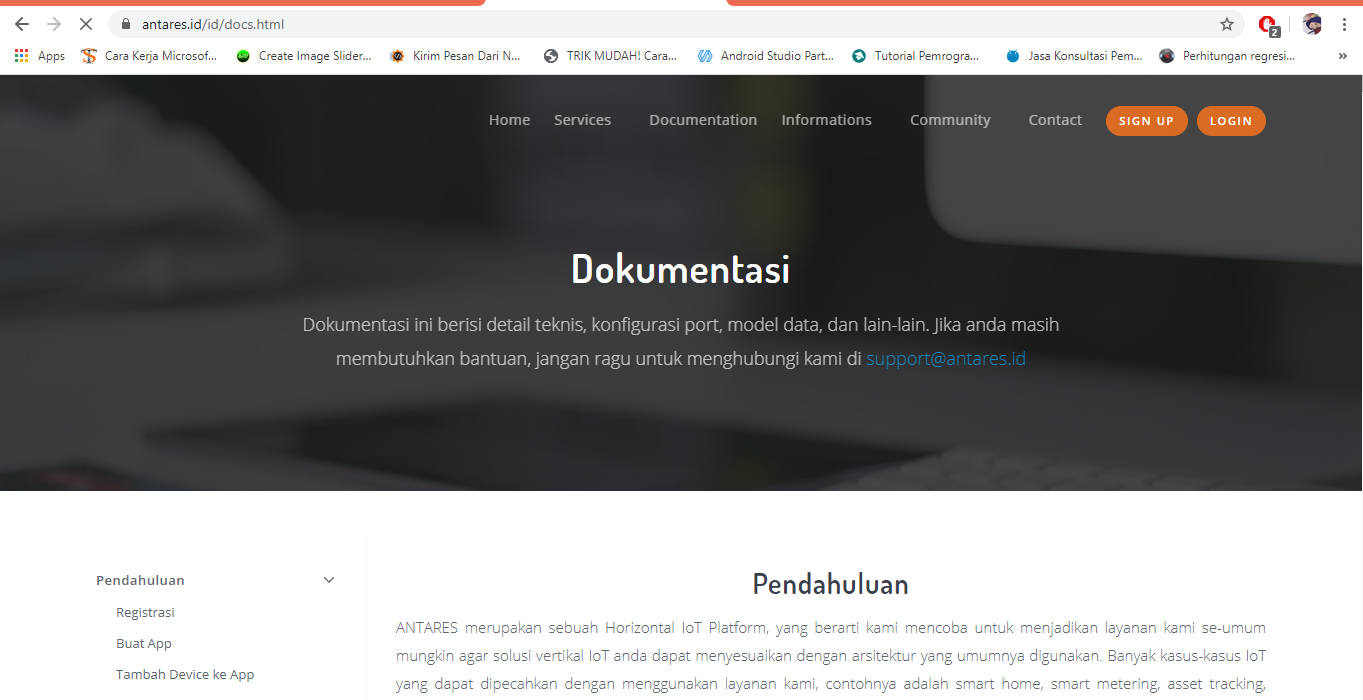
\includegraphics[width=1\textwidth]{figures/antares9.png}
    \caption{Halaman \textit{Documentation}}
    \label{print}
    \end{figure}
    
    \begin{figure}[H]
    \centering
    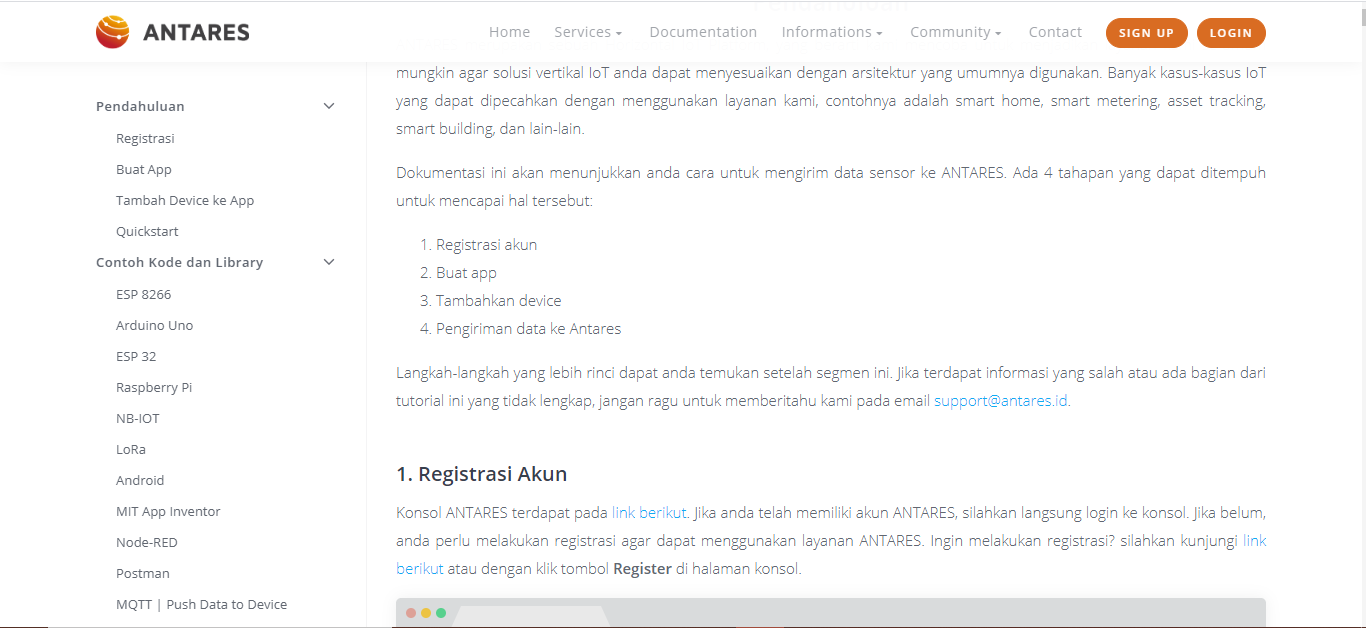
\includegraphics[width=1\textwidth]{figures/antares10.png}
    \caption{Halaman \textit{Documentation}}
    \label{print}
    \end{figure}
    \par Halaman \textit{Documentation} ini merupakan sebuah halaman yang menampilkan tutorial atau penjelasan mengenai penggunaan antares.
    \begin{figure}[H]
    \centering
    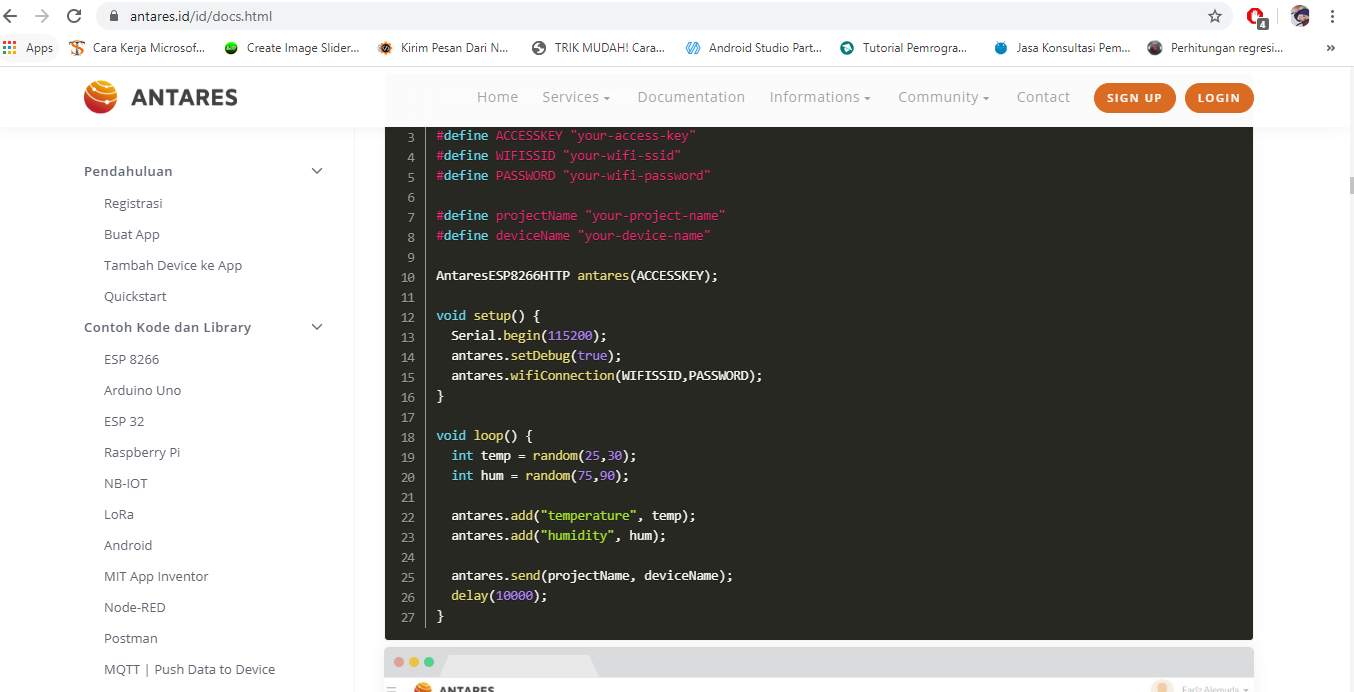
\includegraphics[width=1\textwidth]{figures/antares11.png}
    \caption{Halaman \textit{Documentation} Tutorial}
    \label{print}
    \end{figure}
    
       \begin{figure}[H]
    \centering
    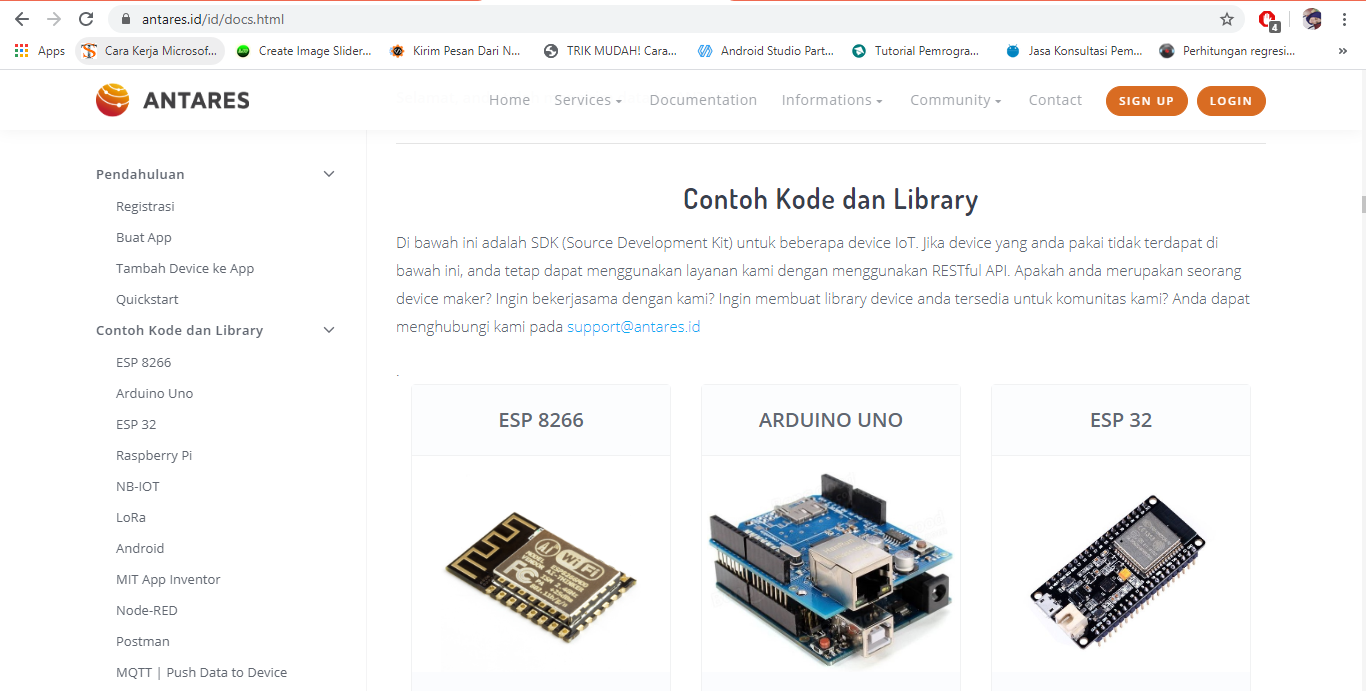
\includegraphics[width=1\textwidth]{figures/antares12.png}
    \caption{Halaman \textit{Documentation}Tutorial}
    \label{print}
    \end{figure}
    \par Pada halaman \textit{documentation} juga terdapat sebuah tutorial mengenai komponen yang dimana menggunakan antares sebagai media penyimpanan datanya. Kemudian pada halaman ini juga menampilkan sebuah contoh kode library yang bisa kita gunakan.
      \begin{figure}[H]
    \centering
    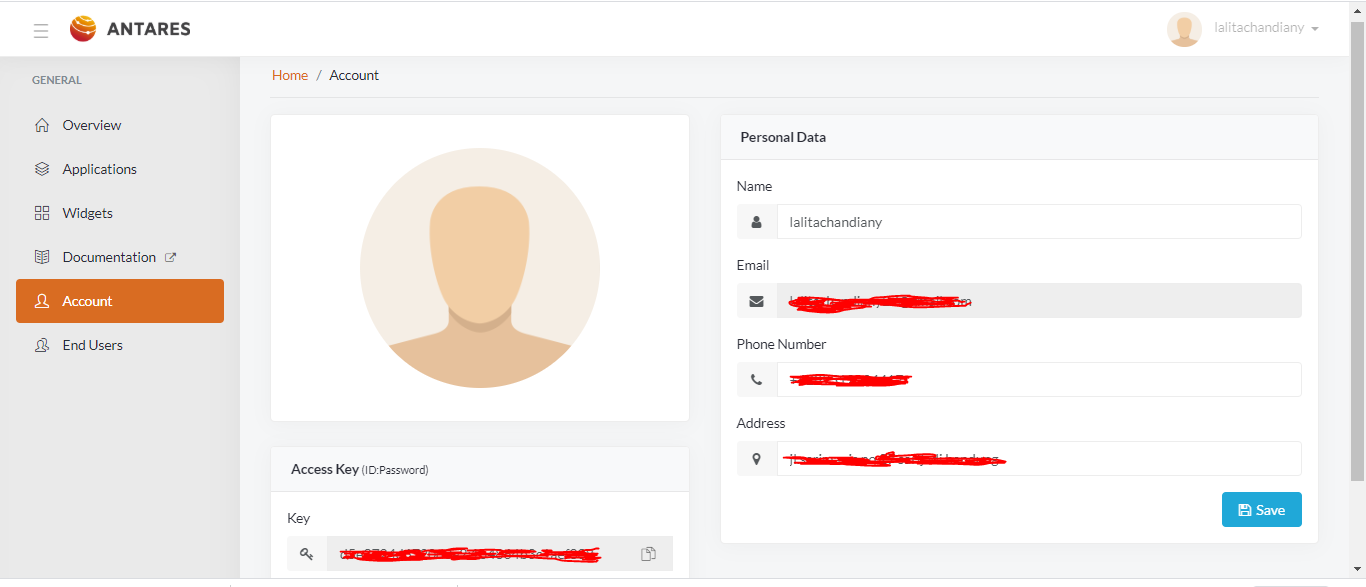
\includegraphics[width=1\textwidth]{figures/antares13.png}
    \caption{Halaman \textit{Account}}
    \label{print}
    \end{figure}
    \par Halaman \textit{account} ini menampilkan suatu informasi pemilik \textit{account} seperti foto profile, \textit{acces key}, \textit{name}, \textit{email}, \textit{phone number}, \textit{address}.
      \begin{figure}[H]
    \centering
    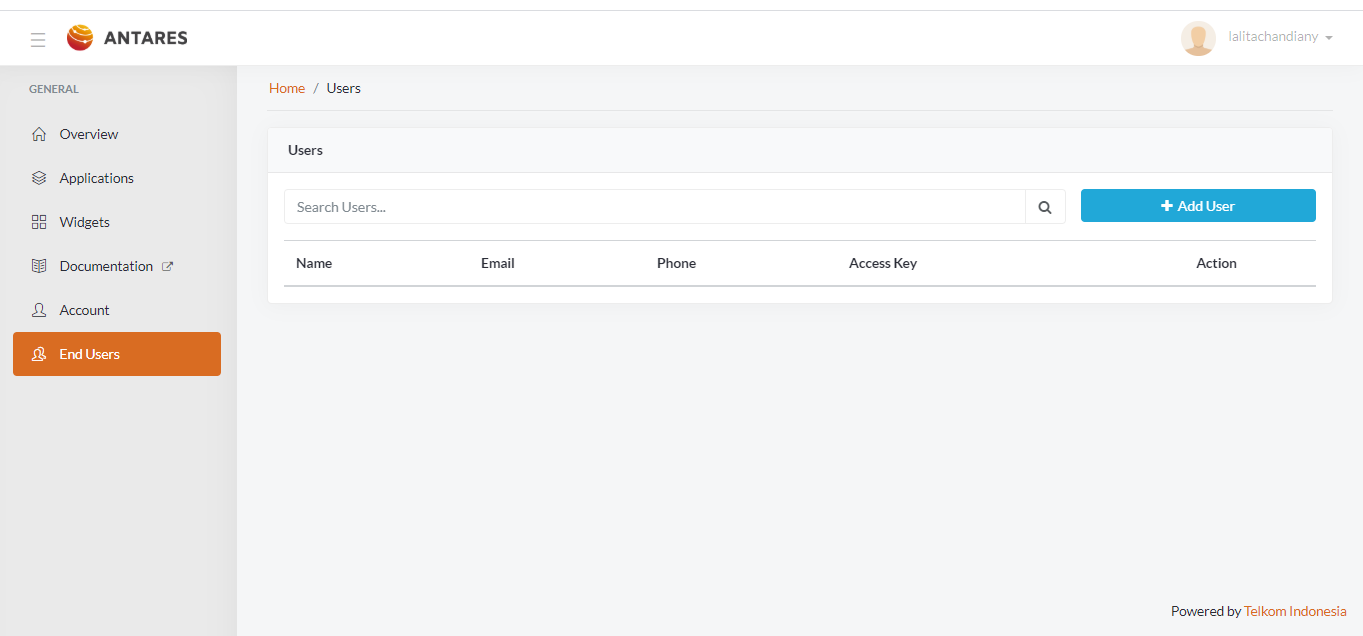
\includegraphics[width=1\textwidth]{figures/antares14.png}
    \caption{Halaman \textit{Enduser}}
    \label{print}
    \end{figure}
    \par Halaman \textit{enduser} berisi mengenai informasi pembuatan user baru dengan cara memasukan \textit{name, email, phone, acces key and action}
\item Memasukan \textit{ Library} antares ke \textit{coding}
\par Sebelum memprogram dan membuat logika tentang antares terlebih dahulu kita harus mendwonload \textit{library} yang akan digunakan dengan cara berikut :
 \begin{figure}[H]
    \centering
    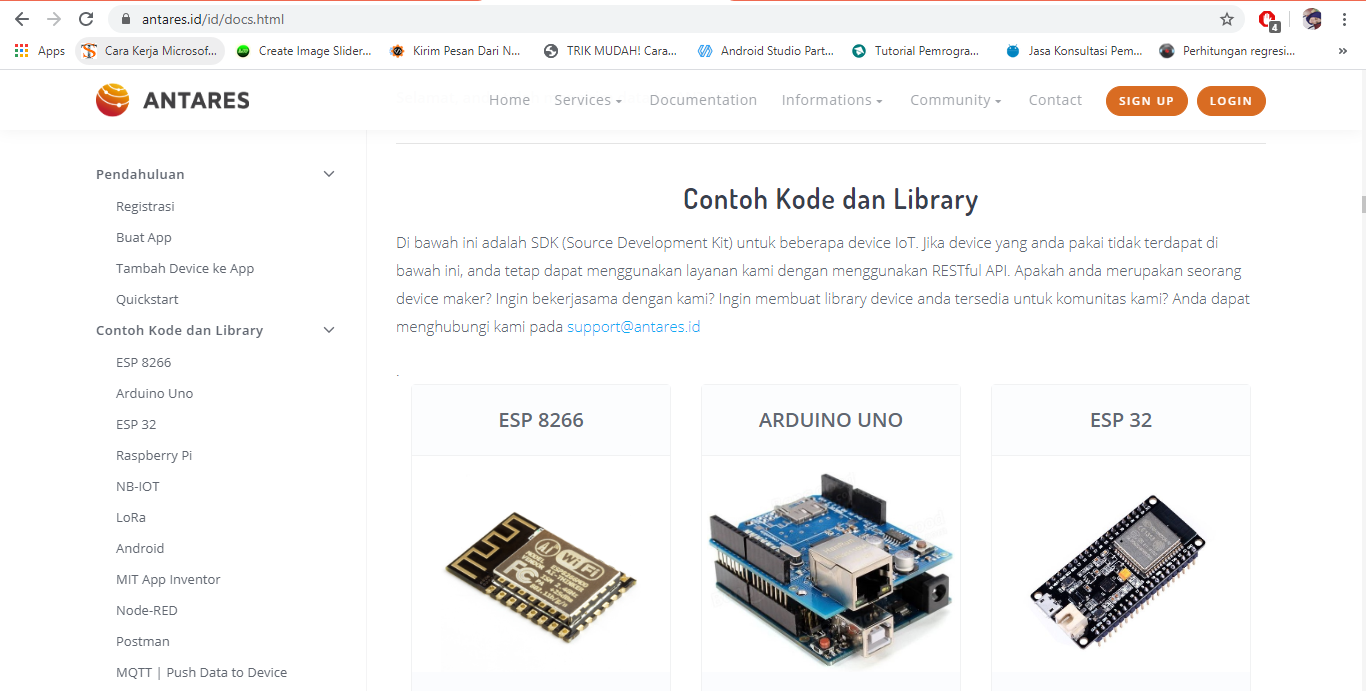
\includegraphics[width=1\textwidth]{figures/antares12.png}
    \caption{Halaman \textit{Documentation}Tutorial}
    \label{print}
    \end{figure}
     
     \par Setelah login keantares pilih menu \textit{documentation} kemudian  pilih esp8266 \textit{go to tutorial}.
      \begin{figure}[H]
    \centering
    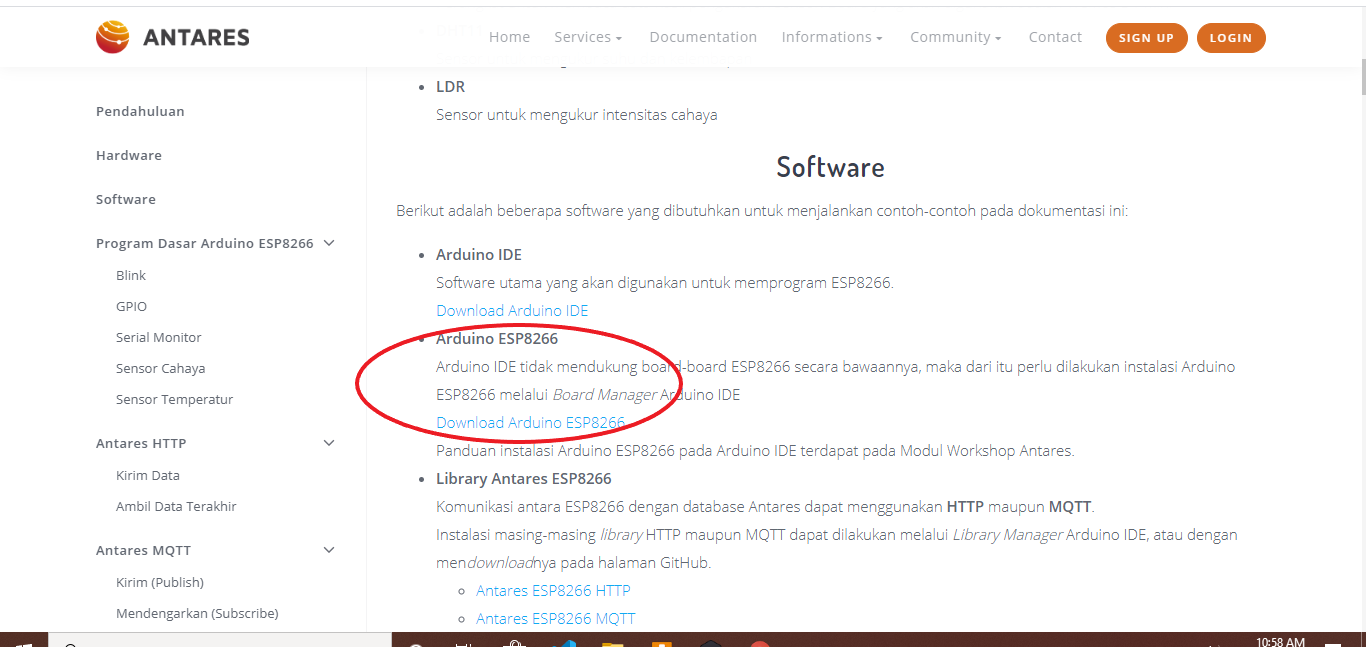
\includegraphics[width=1\textwidth]{figures/antares15.png}
    \caption{Dwonload Library}
    \label{print}
    \end{figure}
    \par Setelah kita memilih \textit{go to tutorial} maka akan muncul tampilan seperti gambar diatas. Lalu pilih atau klik \textit{dwonload} arduino esp8266.
      \begin{figure}[H]
    \centering
    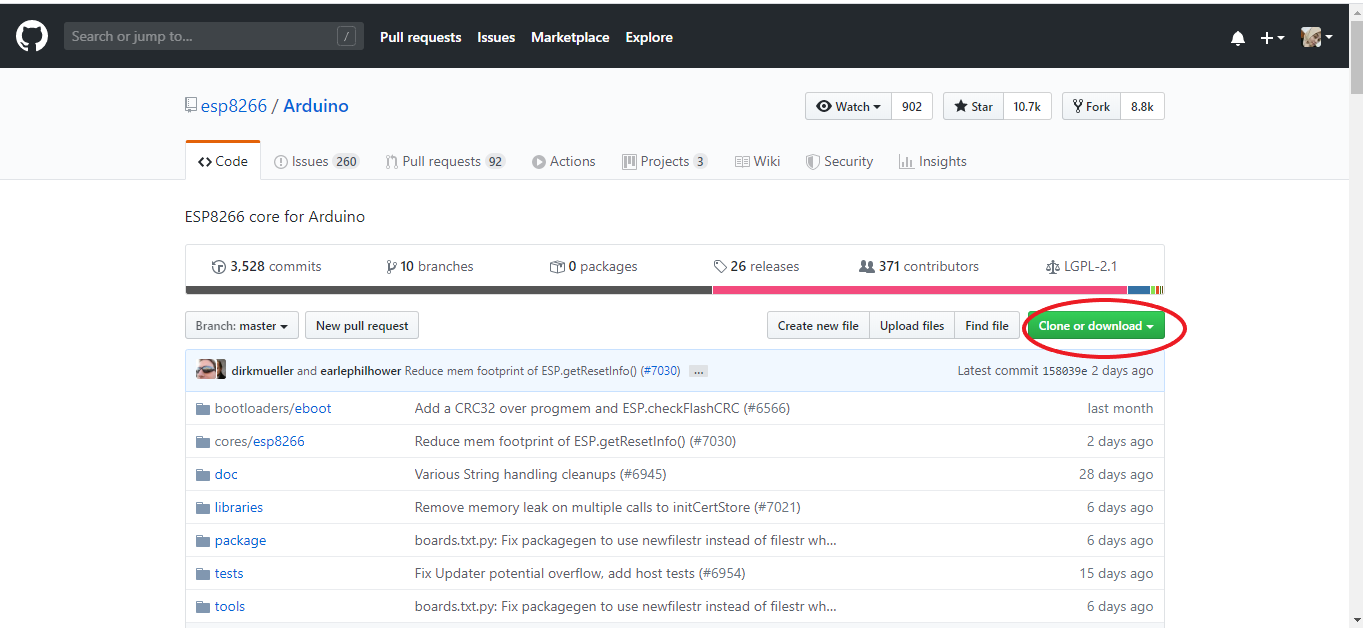
\includegraphics[width=1\textwidth]{figures/antares16.png}
    \caption{Dwonload Library di Github}
    \label{print}
    \end{figure}
    
    \par Ketika kita sudah klik \textit{dwonload} arduino esp8266. Maka Akan muncul tampilan seperti diatas, dimana tampilan tersebut langsung masuk ke repositori di github. Setelah masuk ke github kemudian kita klik menu \textit{clone or dwonload}.
    
      \begin{figure}[H]
    \centering
    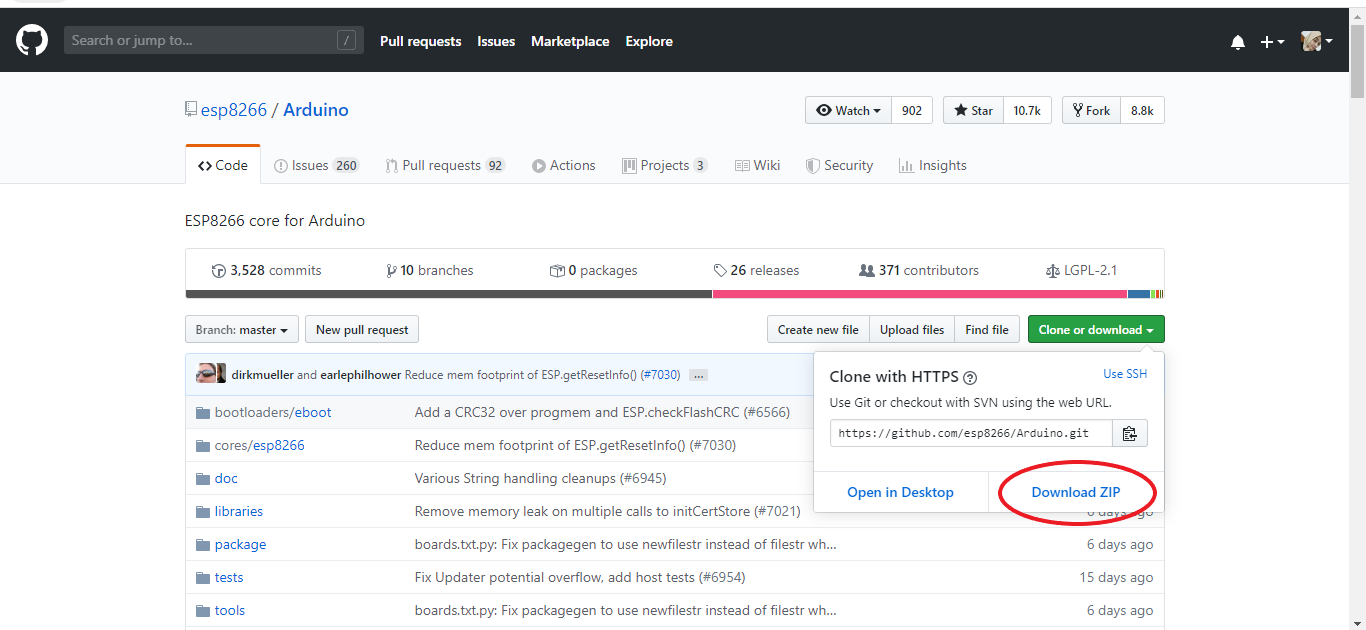
\includegraphics[width=1\textwidth]{figures/antares17.png}
    \caption{Dwonload Library}
    \label{print}
    \end{figure}
     
     \par Ketika menu \textit{clone or dwonload} diklik maka akan muncul dua pilihan seperti pada gambar diatas. Untuk dwonload \textit{library} maka pilih \textit{Dwonload ZIP}.
     
     \par Jika kita ingin kita \textit{import library} menggunakan board manager, maka langkah-langkahnya seperti berikut :
     \begin{figure}[H]
    \centering
    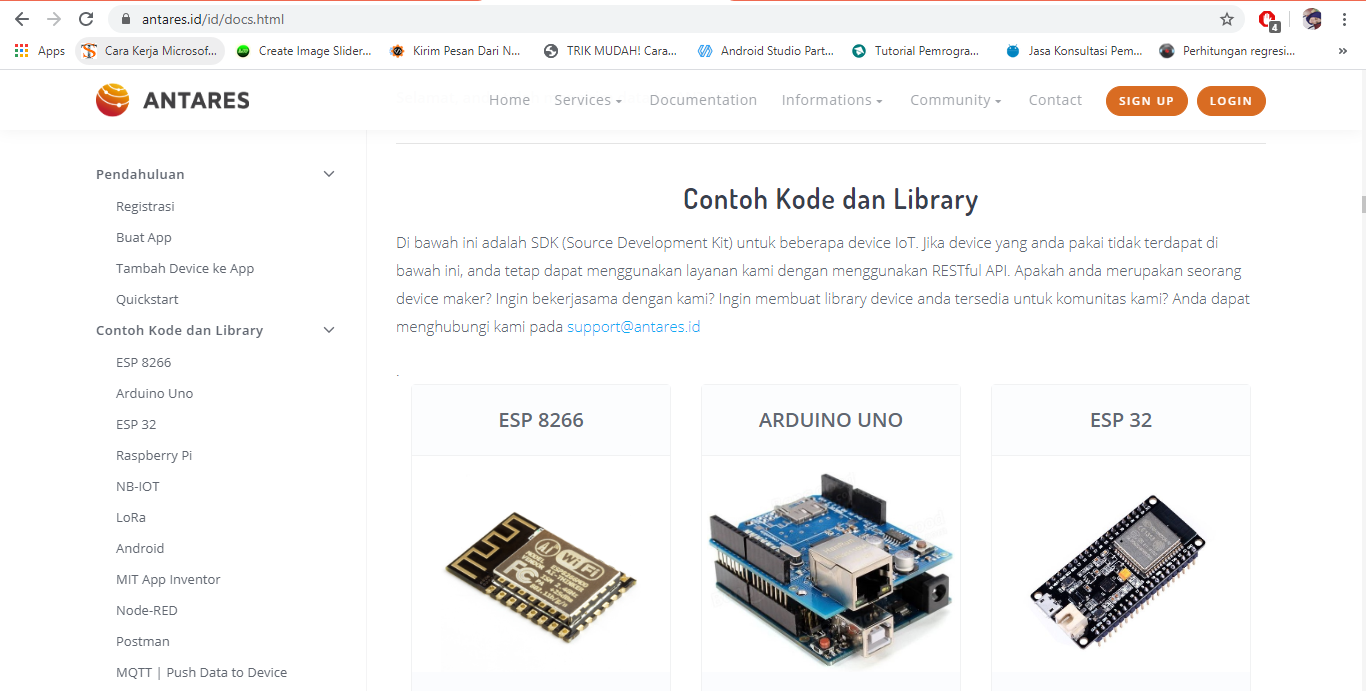
\includegraphics[width=1\textwidth]{figures/antares12.png}
    \caption{Halaman \textit{Documentation}Tutorial}
    \label{print}
    \end{figure}
     
     \par Setelah login keantares pilih menu \textit{documentation} kemudian  pilih esp8266 \textit{go to tutorial}.
      \begin{figure}[H]
    \centering
    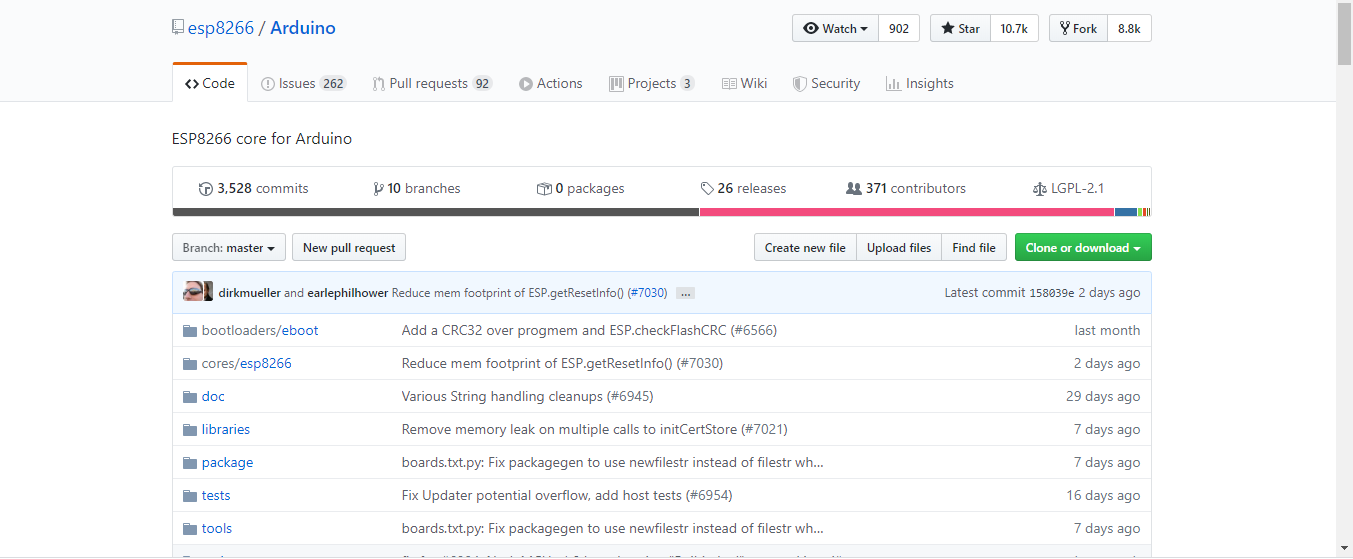
\includegraphics[width=1\textwidth]{figures/antares20.png}
    \caption{Tampilan di Github}
    \label{print}
    \end{figure}
    \par Setelah kita memilih \textit{go to tutorial} maka akan muncul tampilan seperti gambar diatas. Lalu scroll kebawah hingga menenmukan tulisan \textit{contents}.
     \begin{figure}[H]
    \centering
    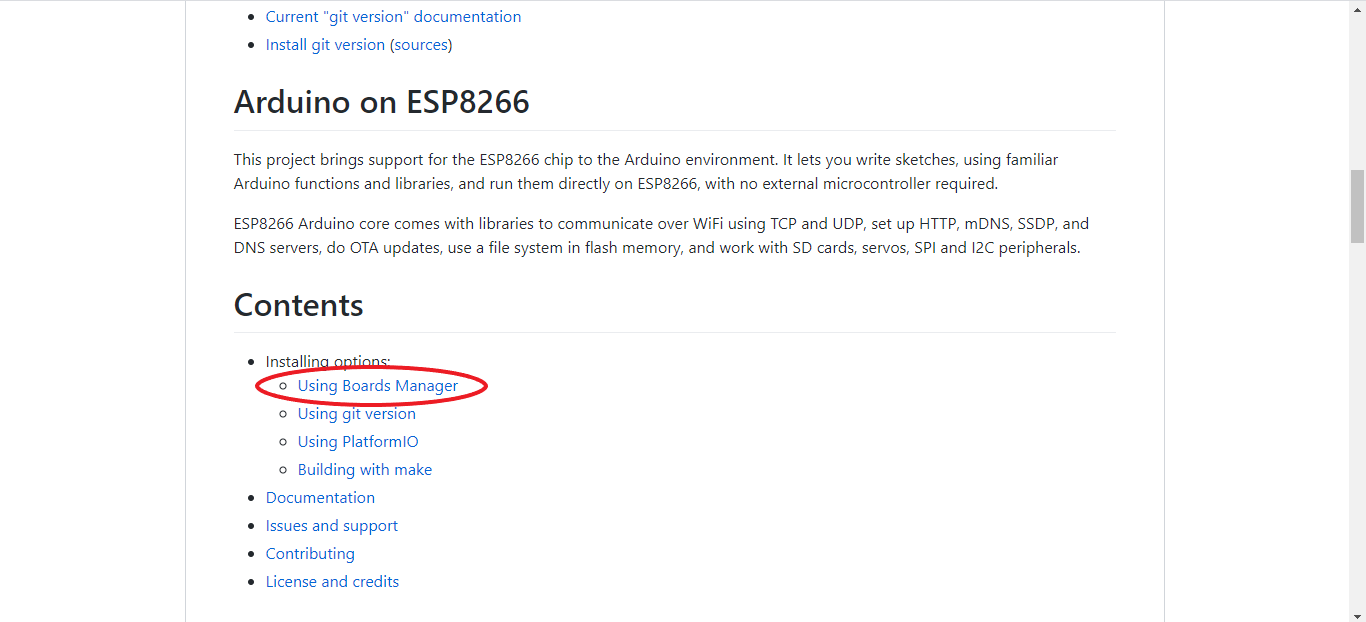
\includegraphics[width=1\textwidth]{figures/antares18.png}
    \caption{Tampilan \textit{content}}
    \label{print}
    \end{figure}
    
    \par Kemudian setelah \textit{scroll} ke bawah hingga menemukan tulisan \textit{content maka} pilih atau klik \textit{using boards manager}.
     \begin{figure}[H]
    \centering
    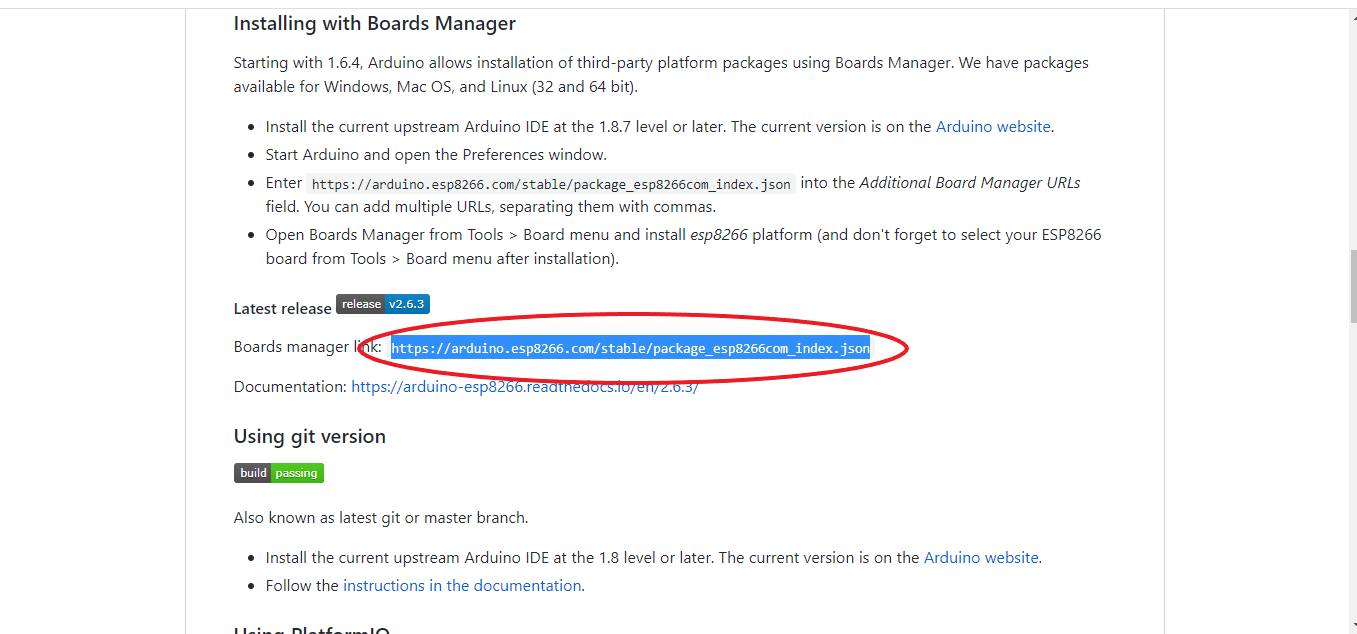
\includegraphics[width=1\textwidth]{figures/antares19.png}
    \caption{Tampilan Using Boards Manager}
    \label{print}
    \end{figure}
    
    \par Ketika klik \textit{using boards manager} maka tampilan yang akan ditampilkan seperti gambar diatas. Kemudian kita copy alamat link yang tertera.
     \begin{figure}[H]
    \centering
    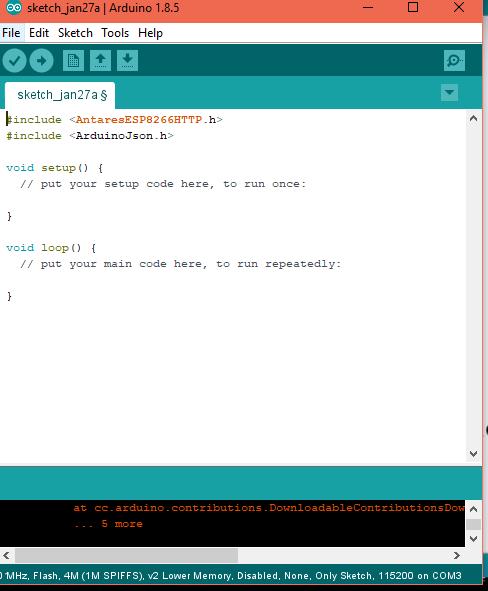
\includegraphics[width=1\textwidth]{figures/manager9.png}
    \caption{Tampilan Arduino IDE}
    \label{print}
    \end{figure}
    
    \par Setelah mengcopy link dari github,Kita terlebih dahulu membuka \textit{software} arduino IDE.
    
    \begin{figure}[H]
    \centering
    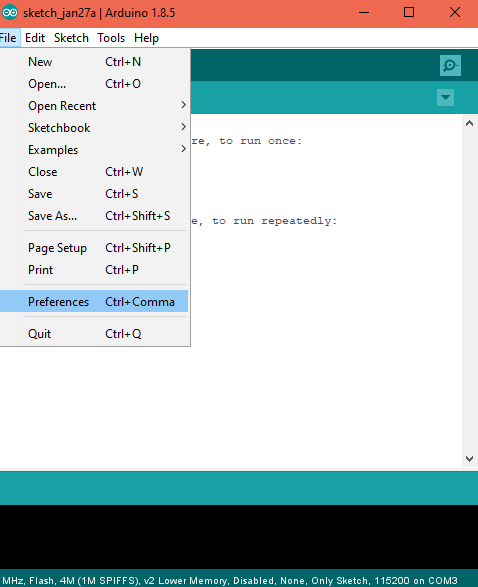
\includegraphics[width=1\textwidth]{figures/managerpre.png}
    \caption{Tampilan Arduino IDE }
    \label{print}
    \end{figure}
    
    \par Ketika arduino IDE telah dibuka. Maka kita pilih File klik Preferencer seperti pada gambar diatas.
    \begin{figure}[H]
    \centering
    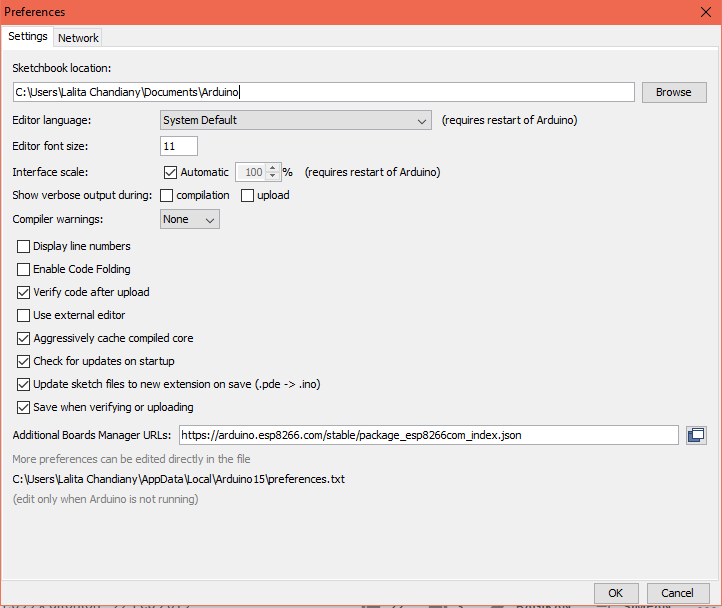
\includegraphics[width=0.7\textwidth]{figures/manager4.png}
    \caption{Tampilan Preferences}
    \label{print}
    \end{figure}
    
    \par Setelah memlih preferences maka tampilannya yang muncul seperti pada gambar tersebut. Kemudian paste alamat url di bagian \textit{Additional Boards Manager URLs} yang sebelumnya di copy dari github dan klik ok.
    \begin{figure}[H]
    \centering
    \includegraphics[width=0.7\textwidth]{figures/managerboar.png}
    \caption{Tampilan Arduino IDE Boards Mnager}
    \label{print}
    \end{figure}
    
    \par Kemudian jika sudah salin alam url nya maka selanjutnya pilih Tools lalu Boards kemudian Boardmanager seperti gambar diatas.
    
    \begin{figure}[H]
    \centering
    \includegraphics[width=1\textwidth]{figures/manager5.png}
    \caption{Tampilan Boards Manager}
    \label{print}
    \end{figure}
    \par Jika kita telah klik boards manager maka akan muncul tampilan boards manager.
    
    \begin{figure}[H]
    \centering
    \includegraphics[width=1\textwidth]{figures/manager6.png}
    \caption{Tampilan Boards Manager Antares}
    \label{print}
    \end{figure}
    \par Ketika tampilan boards manager telah muncul kita scroll ke yang paling bawah. Kemudian install esp8266 dan versinya disesuaikan.
    
    \begin{figure}[H]
    \centering
    \includegraphics[width=1\textwidth]{figures/managelib.png}
    \caption{Tampilan Arduino IDE Include Library}
    \label{print}
    \end{figure}
    
    \par Setelah menginstal esp8266 tahapan selanjutnya kita pilih Skecth lalu Include Library kemudian Manage Library. Seperti pada gambar diatas.
    \begin{figure}[H]
    \centering
    \includegraphics[width=1\textwidth]{figures/manager7.png}
    \caption{Tampilan Library Manager}
    \label{print}
    \end{figure}
    
    \par Jika kita telah klik manage libraries maka akan muncul tampilan seperti gambar diatas.
     \begin{figure}[H]
    \centering
    \includegraphics[width=1\textwidth]{figures/manager8.png}
    \caption{Tampilan Library Manager Antares}
    \label{print}
    \end{figure}
    \par Setelah muncul tampilan manage libraries kemudian ketikan antares pada bagian \textit{search}. Ketika telah memasukan kata antares maka akan muncul \textit{library} antares paling atas lalu install.
    \begin{figure}[H]
    \centering
    \includegraphics[width=1\textwidth]{figures/manageinclude.png}
    \caption{Tampilan Arduino IDE Manage Library}
    \label{print}
    \end{figure}
    
    \par Jika telah menginstall semua library antares yang dibutuhkan, maka hal yang harus dilakukan selanjutnya yaitu menginclude library dengan cara pilih \textit{skecth} lalu \textit{include library} dan pilih Antares ESP8266HTTP.
    
    \begin{figure}[H]
    \centering
    \includegraphics[width=1\textwidth]{figures/manager9.png}
    \caption{Tampilan Arduino IDE Library Antares}
    \label{print}
    \end{figure}
    \par Jika kita sudah mengklik library antares yang telah di dwonload maka akan langsung tertampahkan \textit{code}nya seperti pada gambar diatas.
    \\
    \\
    \item Membuat Project Di Antares
    \par Sebelum membuat sebuah program yang isinya gabungan dari beberapa komponen untuk membuat \textit{prototype} ini , diperlukan terlebih dahulu membuat sebuah \textit{project} atau \textit{application} di antares yang bertjuan untuk menyimpan data yang dibaca oleh sensor jarak. Berikut langkah-langkahnya :
    
     \begin{figure}[H]
    \centering
    \includegraphics[width=1\textwidth]{figures/antares2.png}
    \caption{Tampilan Antares}
    \label{print}
    \end{figure}
    
    \par Hal pertama yang harus dilakukan yaitu masuk ke halaman antares hanya dengan mengetikan urlnya pada browser. Url dari antares yaitu antares.id , ketika kita ketikan url tersebut maka akan muncul tampilan awal antares seperti pada gambar diatas.
    \begin{figure}[H]
    \centering
    \includegraphics[width=1\textwidth]{figures/antares5.png}
    \caption{Tampilan Login Antares}
    \label{print}
    \end{figure}

    \par Kemudian pilih menu login dan akan muncul tampilan login. Masukan gmail dan password yang sudah terdaftar sebelumnya.
    \begin{figure}[H]
    \centering
    \includegraphics[width=1\textwidth]{figures/project1.png}
    \caption{Tampilan Awal Antares}
    \label{print}
    \end{figure}
    
    \par Setelah kita melakukan login akan muncul tampilan awal antares yang disediakan dengan beberapa menu. Untuk membuat sebuah \textit{project} baru atau \textit{application} pilih menu \textit{application}.
    \begin{figure}[H]
    \centering
    \includegraphics[width=1\textwidth]{figures/project2.png}
    \caption{Tampilan Application  Antares}
    \label{print}
    \end{figure}
    
    \par Ketika kita mengklik atau pilih menu \textit{application}, maka kita akan dihadapkan dengan tampilan seperti pada gambar diatas. Setelah itu klik \textit{add aplication} untuk membuat sebuah \textit{project} baru.
     \begin{figure}[H]
    \centering
    \includegraphics[width=1\textwidth]{figures/project3.png}
    \caption{Tampilan Membuat Application  Antares}
    \label{print}
    \end{figure}
    
    \par Setelah meng klik \textit{addapplication}, maka ditampilan selanjutnya harus menggisikan \textit{application name} dan \textit{application ID} dengan nama yang bebas. Disini diberinakan sebuah \textit{application name} dan \textit{application IDnya} monitoring. Karena nantinya data ini akan digunakan sebagai monitoring ketinggian air. Kemudian setelah mengisi semua klik \textit{add}.
    
     \begin{figure}[H]
    \centering
    \includegraphics[width=1\textwidth]{figures/project4.png}
    \caption{Tampilan Application Yang Dibuat}
    \label{print}
    \end{figure}
    
    \par Jika kita sudah membuat sebuah \textit{application} atau \textit{project} , maka akan muncul tampilan seperti gabar diatas. Kemudian klik \textit{AddDevice} untuk membuat sebuah \textit{device} baru .
    
     \begin{figure}[H]
    \centering
    \includegraphics[width=1\textwidth]{figures/project5.png}
    \caption{Tampilan Membuat Device Antares}
    \label{print}
    \end{figure}
    
    \par Gambar 3.65 merupakan sebuah tampilan untuk membuat \textit{device} baru.
    \begin{figure}[H]
    \centering
    \includegraphics[width=1\textwidth]{figures/project6.png}
    \caption{Tampilan Membuat Device Antares}
    \label{print}
    \end{figure}
    \par Setelah itu masukan nama \textit{devicename} disini menggunakan nama "tinggisensor". Dimana untuk nama \textit{device} ini bisa bebas sesuai dengan kebutuhan. Jika sudah mengisi nama \textit{device} klik \textit{add}.
     \begin{figure}[H]
    \centering
    \includegraphics[width=1\textwidth]{figures/project7.png}
    \caption{Tampilan Device Di Application Antares}
    \label{print}
    \end{figure}
    
    \par Sesudah membuat \textit{device} pada \textit{application} maka tampilannya seperti pada gambar diatas. Apabila kita ingin mengetahui isi apa saja yang ada \textit{device} , maka klik nama \textit{devicenya}.
     \begin{figure}[H]
    \centering
    \includegraphics[width=1\textwidth]{figures/project8.png}
    \caption{Tampilan Halaman Device Antares}
    \label{print}
    \end{figure}
    
    \par Pada gambar tersebut merupakan sebuah tampilan \textit{device} tinggisensor. Dimana pada \textit{device}ini datanya masih kosong karna belum disambungkan deng project.
    
    \item Memprogram Komponen Dengan Mengkoneksikan Pada Antares
    
    \par Setelah kita membuat sebuah \textit{project} atau \textit{application} di antares, maka sekarang membuat sebuah program yang datanya bisa di simpan diantares. Dimana data tersebut dapat terkoneksi dengan antares.Dengan cara menambahkan code seperti berikut :
    \begin{enumerate}
        \item Pertama kita harus mengimport library dan menginisiasi pin yang digunakan , dengan cara menambahkan \textit{code} berikut :
        \lstinputlisting{src/nodemcuantares.c}
        
        \item Kedua setelah kita menginisiasi pin yang digunakan yaitu mendefinisikan variabel, dengan menambahkan \textit{code} berikut :
        \lstinputlisting{src/nodemcuantares2.c}
        \par Pada saat pendefinisian variabel harus memasukan \textit{acces key} ,WIFI SSID (nama wifi yang akan dikoneksikan), \textit{password} (kata sandi dari wifi SSID) wifi ini digunakan untuk koneksi nodemcu. Sedangkan untuk \textit{acces key} didapatkan dari antares dengan cara sebagai berikut :
         \begin{figure}[H]
        \centering
        \includegraphics[width=1\textwidth]{figures/Key.png}
        \caption{Tampilan Antares}
        \label{print}
        \end{figure}
    \par Pertama \textit{login} antares ketika muncul halaman utama pilih \textit{users}.
     \begin{figure}[H]
    \centering
    \includegraphics[width=1\textwidth]{figures/key2.png}
    \caption{Tampilan Users Antares}
    \label{print}
    \end{figure}
    
    \par Setelah masuk ke halaman \textit{users copy key} tersebut, kemudian di \textit{paste} dibagian pendefinisian variabel.
    
    \item Ketika telah mendefinisikan varial , saatnya masuk bagian void setup, dimana void setup ini dieksekusi pertamakali dan hanya sekali dieksekusi hanya pada saat program dijalan. Selain itu juga pada bagian void setup ini mengatur \textit{inputan} dan \textit{output} berikut codenya :
    \lstinputlisting{src/nodemcuantares3.c}
        
     \item Jika kita telah membuat voidsetup, saatnya membuat void loop. Dimana void loop ini akan dieksekusi terus menerus ketika program dijalankan . Berikut code daei looping sensro ultrasonic , buzzer dan led.
     \lstinputlisting{src/nodemcuantares4.c}
        
    \item Setelah membuat looping mengenai sensor, buzzer dan led, kemudian membuat code untuk ke antaresnya sebagai berikut :
    \lstinputlisting{src/nodemcuantares5.c}
    \item Terakhir yaitu membuat sebuah code untuk menampilkannya di serial monitor dengan cara membuat code berikut ini :
    \lstinputlisting{src/nodemcuantares6.c}
    
    \par Jika kita gabungkan code dari awal yaitu mengimport library sampedengan menampilkan di serial monitor akan seperti berikut ini :
    \lstinputlisting{src/nodemcuantares7.c}
        
    \end{enumerate}
    
    \par Setelah semuanya komponen di program dan sudah dikoneksi dengan antares saatnya mengupload file dengan cara berikut :
    \begin{figure}[H]
    \centering
    \includegraphics[width=1\textwidth]{figures/upload3.png}
    \caption{Verifikasi Arduiono IDE }
    \label{print}
    \end{figure}
    \par Sebelum mengupload ada baiknya kita memverifikasi terlebih dahulu . Verifikasi ini bertujuan untuk mengecek apakah ada error atau tidaknya. Cara untuk memverifikasi dengan cara klik centang seperti pada gambar diatas.
    
     \begin{figure}[H]
    \centering
    \includegraphics[width=1\textwidth]{figures/upload.png}
    \caption{Upload Arduiono IDE }
    \label{print}
    \end{figure}
     \par Kemudian setelah melakukan verifikasi dan apabila tidak ada error maka langsung untuk mengupload code yang sebelumnya telah dibuat klik gambar panah pada arduino IDE seperti pada gambar diatas.
      \begin{figure}[H]
    \centering
    \includegraphics[width=1\textwidth]{figures/upload2.png}
    \caption{Upload Arduiono IDE }
    \label{print}
    \end{figure}
    \par Jika prosser \textit{upload} sudah selesai , maka akan adanya tulisan \textit{done upload} dibagian pojok kanan bawah.
    
    \par Setelah upload maka semua komponen akan menjalankan perintahnya sesuai code yang telah dibuat sebelumnya. Kemudian untuk melihat data yang dibaca oleh sensor ultrasonik kemudian dikirimkan ke antares sebagai berikut :
      \begin{figure}[H]
    \centering
    \includegraphics[width=1\textwidth]{figures/project1.png}
    \caption{Halaman Utama Antares }
    \label{print}
    \end{figure}
    \par Hal pertama yang harus dilakukan yaitu \textit{login} antares, kemudian akan muncul tampilan seperti gambar diatas dan pilih menu \textit{application}.
      \begin{figure}[H]
    \centering
    \includegraphics[width=1\textwidth]{figures/data.png}
    \caption{Tampilan \textit{Application}}
    \label{print}
    \end{figure}
     
     \par Setelah pilih menu \textit{application} maka akan tampil halaman seperti diatas kemudian pilih \textit{project} yang telah kita buat serta dikoneksikan dengan \textit{project prototype} ini yaitu pilih yang bernama monitoring.
      \begin{figure}[H]
    \centering
    \includegraphics[width=1\textwidth]{figures/data2.png}
    \caption{Tampilan \textit{Project}}
    \label{print}
    \end{figure}
     
     \par Ketika kita telah memilih \textit{projectnya} maka akan masuk ke tampilan yang kita harus memilih \textit{device} yang telah dikoneknsikan sebelumnya yaitu nama \textit{devicennya}  tinggi sensor.
      \begin{figure}[H]
    \centering
    \includegraphics[width=1\textwidth]{figures/data3.png}
    \caption{Tampilan Data Sensor Ultrasonic}
    \label{print}
    \end{figure}
    \par Gambar diatas merupakan sebuah data yang dibaca oleh sensor ultrasonic yang dikirimkan ke antares secara \textit{realtime}.
    
    \item Membuat Notifikasi Melalui Telegram.
    \par Pada \textit{prototype} prediksi ketingian air (PKA) untuk mendeteksi banjir peringatan dini ini menggunakan notifikasi melalui telegram. Notifikasi ini akan dikirimkan ketika sensor membaca jarak ketinggian air kurang dari 5 meter.
    \\
    \par Untuk membuat sebuah notifikasi melalui telegram ini kita perlu memprogramnya melalui arduino IDE. Sebelum memprogramnya kita harus membuat sebuah \textit{bot} ditelegram. Dengan cara berikut :
    \begin{enumerate}
        \item Buka aplikasi telegram kemudikan ketikan BotFather.
         \begin{figure}[H]
    \centering
    \includegraphics[width=1\textwidth]{figures/bot1.png}
    \caption{Tampilan Telegram}
    \label{print}
    \end{figure}
    \\
    \\
    \\
    \\
    \\
    \\
    \\
    \item  Lalu buka BotFather, ketik START.
     \begin{figure}[H]
    \centering
    \includegraphics[width=0.9\textwidth]{figures/bot2.png}
    \caption{Tampilan Bot Telegram}
    \label{print}
    \end{figure}
    
    \item Lalu ketik /newbot , selanjutnya akan diminta memberikan nama bot dan username bot. Jika sudah makan akan muncul Token, seperti yang dilingkari dibawah ini. Simpan Token tersebut.
    \begin{figure}[H]
    \centering
    \includegraphics[width=0.7\textwidth]{figures/bot3.png}
    \caption{Tampilan Bot Telegram}
    \label{print}
    \end{figure}
     \begin{figure}[H]
    \centering
    \includegraphics[width=0.9\textwidth]{figures/bot4.png}
    \caption{Tampilan Bot Telegram}
    \label{print}
    \end{figure}
        
    \item Selian BotFather kita juga haru mengetahui idnya yaitu cari IDBot.
     \begin{figure}[H]
    \centering
    \includegraphics[width=1\textwidth]{figures/bot5.png}
    \caption{Tampilan IDBot Telegram}
    \label{print}
    \end{figure}
    
    \item Klik /start , lalu ketik /getid. Nanti akan muncul id telegram kamu seperti yang dibawah ini:
    \begin{figure}[H]
    \centering
    \includegraphics[width=0.9\textwidth]{figures/bot6.png}
    \caption{Tampilan IDBot Telegram}
    \label{print}
    \end{figure}
        
    \begin{figure}[H]
    \centering
    \includegraphics[width=0.9\textwidth]{figures/bot7.png}
    \caption{Tampilan IDBot Telegram}
    \label{print}
    \end{figure}
    \end{enumerate}
    \par Setelah membuat bot dan juga sudah mengetahui Token dan id telegram agan. Selanjutnya yang tidak kalah penting perlu masuk ke Bot yang sudah buat dan klik /start.
    \begin{figure}[H]
    \centering
    \includegraphics[width=0.7\textwidth]{figures/bot8.png}
    \caption{Tampilan Bot Monitoring Di Telegram}
    \label{print}
    \end{figure}
     
 \par Setelah bot dibuat maka selanjutnya kita harus mendwoload libriray untuk telegram. Kita dapat mendwonloadnya di url https://www.dropbox.com/s/2rlrg8kcy\\yx7i3o/CTBot.zip untuk ctbot dan https://www.dropbox.com/s/g9ycw3o3uv7cg\\z7/ArduinoJson.zip untuk arduino json.
   \begin{figure}[H]
    \centering
    \includegraphics[width=0.7\textwidth]{figures/bot9.png}
    \caption{Tampilan Dwonload CTbot}
    \label{print}
    \end{figure}
        
    \begin{figure}[H]
    \centering
    \includegraphics[width=0.9\textwidth]{figures/bot10.png}
    \caption{Tampilan Dwonload Arduino Json}
    \label{print}
    \end{figure}
    
    \par Setelah mendwonload maka saatnya memprogram melalui arduino IDE yaitu sebagai berikut :
    \begin{enumerate}
     \item Langkag pertama yaitu \textit{import} library yang telah didwonload. Sehingga aka muncul secara otomatis code berikut :
    \lstinputlisting{src/bot.c}
    \item Kemudian menginisiasi sebagai berikut kodenya. 
    \lstinputlisting{src/bot2.c}
    \item Kemudian mendefinisikan variabel.
    \lstinputlisting{src/bot3.c}
        
    \item Membuat sebuah inputan maupun outputan dibagian void setup.
    \lstinputlisting{src/bot4.c}
        
    \item Membuat Json nya aga dapat mengirimkan notifikasi melalui telegram.
    \lstinputlisting{src/bot5.c}
    \item Membuat void json nya dengan code sebagai berikut :
    \lstinputlisting{src/bot6.c}
    \item Jika \textit{code}nya digabungkan dari awal sampai menggunakan bot telegram yaitu sebagai berikut :
    \lstinputlisting{src/bot7.c}
    \end{enumerate}
    
     \begin{figure}[H]
    \centering
    \includegraphics[width=0.9\textwidth]{figures/notif.png}
    \caption{Tampilan Notifikasi DI Telegram}
    \label{print}
    \end{figure}
    \par Setelah membuat code untuk notifikasi di telegram. Selanjutnya upload program tersbut untuk mengetahui tidak error jika tidak error aka megirimkan notifikasi awas banjir. Apabila sensor ultrasonik membaca jarak ketinggian air kurang dari 5 meter. Gambar diatas merupakan isi notifikasi dari bot telegram yang sebelumnya sudah dibuat.
    
 
\end{enumerate}